% arara: pdflatex
% arara: pdflatex
% arara: pdflatex

% options:
% thesis=B bachelor's thesis 
% thesis=M master's thesis
% czech thesis in Czech language 
% slovak thesis in Slovak language
% english thesis in English language 
% hidelinks remove colour boxes around hyperlinks  
 
\documentclass[thesis=B,czech]{FITthesis}[2019/12/23]
  
\usepackage[utf8]{inputenc} % LaTeX source encoded as UTF-8
\usepackage{adjustbox}   
\usepackage{listings}
\usepackage{dirtree}   
\usepackage{graphicx}
\usepackage{pdfpages}   
\usepackage{subcaption}
\usepackage{rotating}

% \usepackage{amsmath} %advanced maths 
% \usepackage{amssymb} %additional math symbols
 
\usepackage{dirtree} %directory tree visualisation
\usepackage{hyperref}   
\usepackage{minted}   
    
% % list of acronyms
% \usepackage[acronym,nonumberlist,toc,numberedsection=autolabel]{glossaries}
% \iflanguage{czech}{\renewcommand*{\acronymname}{Seznam pou{\v z}it{\' y}ch zkratek}}{}
% \makeglossaries

\newcommand{\tg}{\mathop{\mathrm{tg}}} %cesky tangens
\newcommand{\cotg}{\mathop{\mathrm{cotg}}} %cesky cotangens
\newcommand\tstrut{\rule{0pt}{2.4ex}}
\newcommand\bstrut{\rule[-1.0ex]{0pt}{0pt}}

% % % % % % % % % % % % % % % % % % % % % % % % % % % % % % 
% ODTUD DAL VSE ZMENTE
% % % % % % % % % % % % % % % % % % % % % % % % % % % % % % 

\department{Katedra softwarového inženýrství}
\title{IoT platforma s webovým rozhraním}
\authorGN{Martin} %(křestní) jméno (jména) autora
\authorFN{Skalický} %příjmení autora
\authorWithDegrees{Martin Skalický} %jméno autora včetně současných akademických titulů
\author{Martin Skalický} %jméno autora bez akademických titulů
\supervisor{Ing. Jiří Mlejnek}
%\acknowledgements{Doplňte, máte-li komu a za co děkovat. V~opačném případě úplně odstraňte tento příkaz.}
\abstractCS{Tato práce se zabývá porovnáním aktuálních IoT platforem na trhu pro domácnosti a následným návrhem vlastního řešení včetně implementace. Základním pilířem celého řešení je definice schématu, dle kterého každé zařízení popíše své schopnosti a uživateli se následně zobrazní příslušné rozhraní vygenerované ná základě jeho dovedností. Platforma je určena pro domácí kutily a technické entuziasty, kteří chtějí mít svá zařízení pod jednotným rozhraním. Uživatelské rozhraní je realizováno progresivní webovou aplikací. Součásti práce je také tvorba zařízení založeného na čipu ESP8266 pro měření teploty v udírně, na kterém je demonstrováno jeho zapojení do Platformy.}

\abstractEN{This thesis focuses on a comparison of existing IoT platforms available on the market for smart homes and subsequent design of a custom solution including its implementation. The backbone of whole solution is definition of a scheme that will be used by every connected device to describe its capabilities. User is presented to a generated interface based on the description of connected devices. Platform is designed for use by technical enthusiasts, who want to control all their devices through single interface. The user interface is realized as progressive web app. Part of the thesis also deals with a design and manufacturing of smart device based on chip ESP8266 with purpose of measuring a temperature in a smokehouse. On this smart device the thesis also demonstrates a connection of a device to the platform.}

\placeForDeclarationOfAuthenticity{V~Praze}
\declarationOfAuthenticityOption{4} %volba Prohlášení (číslo 1-6)
\keywordsCS{IoT Platforma, OpenSource, implementace IoT Platformy, PWA, MQTT, ESP8266}
\keywordsEN{Nahraďte seznamem klíčových slov v angličtině oddělených čárkou.}
% \website{http://v3.iotplatforma.cloud} %volitelná URL práce, objeví se v tiráži - úplně odstraňte, nemáte-li URL práce

\begin{document}

% \newacronym{CVUT}{{\v C}VUT}{{\v C}esk{\' e} vysok{\' e} u{\v c}en{\' i} technick{\' e} v Praze}
% \newacronym{FIT}{FIT}{Fakulta informa{\v c}n{\' i}ch technologi{\' i}}

\begin{introduction}
    %sdělit že téma je nové, aktuální, je ho potřeba řešit, komu to bude prospěšné, proč jsme si ho zvolili - vypadá dobře oborová motivace -> vyřešení daného problému někomu pomůže (ideálně nějaké komunitě), sdělit povrchově čím se zabývá práce ->rozvedení v kapitole Cíl, pak na konci úvodu stručné představení práce, aby si čtenář udělal představu jak budu postupovat

    Internet věcí je velmi diskutovaným tématem posledních několika let, ale jeho vývoji předcházela spousta trnitých cest a slepých uliček. Pod kouzelnou zkratkou IoT se pro mnohé skrývá příslib pokroku od chytré domácnosti až po revoluci v průmyslu. Internet věcí je označení pro síť fyzických zařízení, která spolu dokáží komunikovat ať už napřímo nebo pomocí prostředníka. Pro efektivní správu se zařízení připojují k centrální Platformě, která sbírá data z jednolivých zařízení a dle definovaných pravidel zařízením posílá příkazy. Například v domácnosti čidlo pohybu zaregistruje příchod majitele domů a Platforma v reakce zapne vytápějí. Současně poskytuje uživatelské rozhraní, pomocí kterého lze jednotlivá zařízení přímo ovládat a definovat scénáře, na základě kterých se vykonává automatizace jako uvedené automatické zapnutí vytápějí. Platforma je tedy nedílnou součástí světa IoT a od jejích funkcí se odvíjí možnost využití plného potenciálu.

    Na trhu již dnes existují hotová řešení, ale je velmi problematické se mezi nimi zorientovat a často bývají velmi drahá. Důvodem vzniku této práce je negativní osobní zkušenost a vysoké poplatky komerčních řešení s cílem vytvoření dostupné otevřené Platformy pro technické entuziasty a bastlíře, kteří si chtějí jako já vytvářet levná zařízení a jednoduše je spravovat/ovládat.

    Teoretická část práce se věnuje rešerži aktuálních řešení na trhu, jejich vzájemným porovnáním a návrhem vlastního. Praktická část se zaměřuje na implementaci a nasazení vlastního řešení.

    %představit koncepci koncovích zařízení
    %využití - sledování vláhy, zalévání, udírna, ovládání hlasem

    % Takovýchto řešení již dnes existuje celá řada a podíváme se na výhody a nevýhody těch nejznámějších řešení jak z komerčního, tak i OpenSource světa.
    % Následně se budeme věnovat návrhu vlastního řešení s důrazem na bezpečnost, kterou stále spousta výrobců opomíjí. Moje řešení bude mít webové rozhraní, které umožní ovládání ze všech běžných zařízení bez nutnosti vytvářet nativní aplikace.


\end{introduction}

\chapter{Cíl práce}
% návrh vlastní platformy, cíleno pro kutily, bezpečnost pochybná u komerčních řešení -> já chci mít velkou, moje řešení bude více decentralizované
Cílem této práce je navrhnout a implementovat řešení IoT platformy, která bude primárně určena pro domácí kutily, kteří mohou k platformě připojit tzv. DIY (\uv{Udělěj si sám}) zařízení. Platforma tedy bude muset být univerzální, tak aby umožnila připojení různorodých zařízení. Uživatelské rozhraní bude realizováno formou webové aplikace, která umožní sledování a ovládání jednotlivých zařízení.

Hlavním přínosem bude vytvoření alternativy k již existujícím řešením pro ty, kteří hledají vyšší bezpečnost a nižší cenu než často nabízí komerční řešení. Platforma bude koncipována tak, aby si uživatel přidal zařízení na jedno kliknutí a mohl ho ihned ovládat bez nutnosti často zdlouhavých konfigurací, ke kterým zpravidla potřebuje hlubší znalosti. Výsledná platforma bude uvolněna pod OpenSource licencí s možností vlastního hostingu.

Vzhledem k rozsahu Bakalářské práce není cílem nahradit existující řešení, která již obsahují velké množství funkcí, ale vytvořit možnou alternativu a demonstrovat složitost vytvoření celého řešení za použití moderních technologií.



\chapter{Analýza}
Tato kapitola se zabývá definicí IOT Platformy, analýzou již existujících řešení a následně stanovením požadavků na řešení vlastní.


\section{Definice IOT Platformy}
"IOT Platforma je více vrstvá technologie, která umožňuje přímočaré zajištění, ovládání a automatizaci připojených zařízení ve světě internetu věci. Zjednodušeně propojuje Váš hardware, jakkoli rozdílný, do cloudu s možností různorodé konektivity, obsahuje bezpečnostní mechanizmy a široké možnosti pro zpracování dat. Pro vývojáře IoT Platforma nabízí předpřipravené funkce, které vysoce zvyšují rychlost vývoje aplikací pro připojená zařízení a řeší škálování a kompatibilitu napříč zařízeními". (překlad autora) \cite{kaaproject}

\subsection{Definice pojmů}
V této sekci jsou vysvětleny pojmy, které budou použity v následujících kapitolách.

\begin{itemize}
    \item \textbf{Platforma} - Platformou se rozumí programové řešení umožňující propojení různorodých zařízení a jejich následnou obsluhu
    \item \textbf{Koncové zařízení} - Zařízení, které dokáže komunikovat po síti a nabízí nějakou funkcionalitu (např. měření teploty nebo ovládání světla)
    \item \textbf{Bridge} - Síťové zařízení, které funguje jako prostředník mezi koncovými zařízeními a jinou sítí. Agreguje jednotlivá zařízení a nabízí rozhraní pro komunikaci s nimi.
\end{itemize}


\section{Vlastnosti}
Tato sekce se věnuje definice klíčových vlastností IoT platformy: způsobu komunikace se zařízeními, možnostmi automatizace, bezpečností a cílovou skupinou.

\subsection{Komunikace}
Komunikaci mezi zařízeními lze realizovat fyzickým propojením či bezdrátově. Drátové propojení je finančně nákladnější a především znamená obrovský zásah do stávající infrastrukturu domu, využívá se nejčastěji v nové výstavbě, protože nabízí vyšší spolehlivost a odolnost. Bezdrátová komunikace se naopak používá při instalace do stávajících domů nebo z důvodů ušetření nákladu a v této práci se ji budeme věnovat blíže. Lze ji rozdělit do dvou základních kategorií:
\begin{itemize}
    \item \textbf{Centralizované} - Každé zařízení komunikuje pouze s jedním centrálním prvkem, přes který jde veškerá komunikace. Mezi nejznámější technologii tohoto typu patří Wifi.
    \item \textbf{Decentralizované} - V této síti komunikují zařízení přímo s ostatními bez jakéholiv prostředníka. Pokud nelze s cílovým zařízením komunikovat přímo, tak využijí ostatní pro předání zprávy. Síť je díky tomu mnohem odolnější vůči výpadkům, protože zde není tzv. \uv{jediný bod selhání} (single point of failure). Zpravidla mívá nižší datovou propustnost a je složitější pro nasazení a následnou správu. Velkou výhodou je snadnější rozšiřitelnost pokrytí, protože každé přidané zařízení rozšiřuje signál a tímto způsobem lze zařízení řetězit. Pro podrobější popis doporučuji \cite{mesh}.
\end{itemize}
Vzhledem k rozšířenosti Wifi, kterou dnes najdeme v každé domácnosti, se přirozeně nabízí její využití i pro internet věcí. A k tomu v posledních letech opravdu došlo. Díky extrémně levnému chipu ESP8266, který se dnes i u nás v ČR dá koupit za 70 Kč \cite{hadex}, došlo k masivní penetraci trhu s chytrými zařízeními využívající právě Wifi. Bohužel tato technologie má i svá negativa, největšími jsou spotřeba elektrické energie a limit maximálního počtu připojených zařízení na jeden centrální prvek (řádově desítky). Vysoká spotřeba je dána nutností časté komunikace jen kvůli udržení aktivního spojení a proto je možné provozovat zařízení na baterie pouze v jednotkách dnů, maximálně týdnů.

Pro bateriový provoz vznikly speciální sítě, které na rozdíl od Wifi umožní přenos v desítkach kb za sekundu (tisícina rychlosti běžné Wifi), ale jsou energeticky mnohem úspornější \cite{Wifi-vs-ble} (umožnují provoz až desítky let na malou baterii), mají mnohonásobně větší dosah a umožňují propojení mnohem většího počtu zařízení (stovky).

Poměrně rozšířenými z centrálně orientovaných sítí jsou u nás SigFox a LoRa. SigFox je komerční řešení, kde se platí za každé připojené zařízení \cite{sigfox-price}. Oproti tomu síť LoRa používá otevřený standard pro komunikaci LoRaWAN \cite{lora}. Protože se jedná o otevřený standard, tak kdokoliv může vytvořit a provozovat kompatibilní zařízení \cite{lora}. Samozřejmně také lze využití komerční infrastrukturu, kam lze připojit svá zařízení za poplatek, tuto službu nabízí např. České radiokomunikace \cite{cra}, ale díky otevřenosti má každý možnost si za pár tisíc postavit vlastní GateWay (centrální prvek) a provozovat libovolná zařízení bez jakýchkoliv poplatků a prostředníků.

%https://thesmartcave.com/z-wave-vs-zigbee-home-automation/
Z decentralizovaných sítí jsou na trhu poměrně rozšířené Zigbee a Z-Wave. Zigbee je otevřený standard, který dokáže pracovat, jak v pásmu 2.4GHz, tak i 900 MHz \cite{zigbee}. Nemá omezení na maximální počet zařízení zřetězených za sebou a dokáže vytvořit síť skládající se až ze 65 tisíc zařízení \cite{zigbee}. Z-Wave je naopak uzavřený standard, který funguje pouze v pásmu 800-900 MHz \cite{zwave}. Limituje maximální počet přeposlání zprávy na 4 a podporuje síť o velikosti až 256 zařízení \cite{zwave}. Obě sítě jsou energeticky velmi úsporné a umožňují běh zařízení na obyčejnou knoflíkovou baterii po dobu až několika let \cite{zigbee, zwave}.

\subsection{Automatizace}
%https://www.iot-now.com/2020/06/10/98753-iot-home-automation-future-holds/
Automatizace je ve světě IoT pravděpodobně nejdůležitějším tématem a každá IOT Platforma by ji měla umožňovat, protože dává možnost využít zařízení úplně novým způsobem \cite{what-future-hold}. Principiálně se jedná o možnost definování reakcí na jednotlivé události. Událostí může být např. změna teploty, otevření okna nebo detekce pohybu a reakce změna stavu zařízení - zhasnutí světla nebo zapnutí televize \cite{what-future-hold}. V podstatě jediným limitem je zde lidská představivost. Modelový scénář:

Představme si moderní dům, ve kterém jsou všechny věci, které nás napadnou chytré, což s dnešními technologickými možnostmi není sci-fi, ale naopak možná realita. Majitel domu, říkejme mu Joe, přichází večer unavený domů a odemyká dveře. Vejde dovnitř a světlo na chodbě a v kuchyni již svítí. Jde přímo do kuchyně, protože po dlouhém dni v práci má hlad a usedá s jídlem ke stolu. Nemá rád ticho, tak řekne: \uv{Alexo, zapni hudbu} a ze sterea se spustí Beethoven, protože Alexa ví, že je to Joeův oblíbený skladatel klasické hudby. Joe cítí, jak se po místnosti rozprostřívá příjemné teplo ze zapnuté klimatizace. Po večeři odchází do druhého patra do koupelny. Samozřejmně se nemusí starat o zapnuté stereo ani světla, protože se vše samo vypne, jakmile odejde. Ve sprše pustí vodu, která má automaticky teplotu nastavenou specificky dle Joeovi preference 36 °C i přes to, že 20 min před ním se sprchovala jeho přítelkyně, která si libuje v teplejší vodě. Po sprše jde do ložnice a ulehá do postele, zatímco se kontroluje, jestli jsou všechny dveře zamčené, okna zavřená a zapíná se alarm pro případný pohyb ve spodním patře. A jak mohlo být vše uzpůsobené Joeovím preferencím a vše zapnuté ještě před jeho vstupem do domu? Protože zvonek u dveří má kameru s rozpoznáváním obličeje - Joea tedy poznal a vše nastavil.

Takto tedy může vypadat automatizace v domácnosti, která zpříjemní život a odprostí Vás od spousty všedních věcí. Vše nastavené dle osobních preferencí a to nejen určité rodiny, ale na úrovni jednotlivců v domácnosti.


\subsection{Bezpečnost a soukromí}
Při výběru Platformy by důležitým kritériem měla být bezpečnost. Na první pohled se to však nemusí zdát být důležité. Co se může stát, když bude s platformou komunikovat čidlo pohybu a někdo se dokáže dostat k těmto údajům? Například pro zloděje mohou být taková data zlatý důl, protože bude přesně vědět, kdy je dům prázdný.

Bezpečnost je potřeba zde sledovat hned na několika faktorech. Prvním je komunikační médium. Pokud zařízení komunikují bezdrátově, tak by komunikace měla být šifrovaná, aby se nedala jednoduše odposlechnout. Druhým faktorem je bezpečnost samotné platformy. Pokud je platforma dostupná pouze na interní síťi v domácnosti, tak bezpečnost na první pohled ohrožená není. Když se ale zamyslíme nad tím, kolik dnes máme doma chytrých zařízení, tedy takových, které dokáží komunikovat přes internet, tak zjistíme, že jich je velké množství. Dnes např. chytrou televizi má doma téměř každý a je otázkou, na kolik věříme výrobcům těchto zařízení, že kladou důraz na jejich bezpečnost. Stačí, aby nějaký vir napadl naší televizi či jiné zařízení a případný útočník má plný přístup k platformě pouze získáním přístupu do interní sítě. Proto by platforma měla využívat alespoň systém pro identifikaci, ideálně i autentifikaci a to nejen v případě, že je přístupná z internetu, ale i z vnitřní sítě.

\subsection{Cílová skupina}
Internet věcí lze využít napříč všemi sférami. Od jednoduché meteostanice, která měří teplotu, přes tvz. chytrou domácnost, kdy Vám lednička pošle nákupní seznam podle chybějících potravin, přes využití v průmyslu pro sběr různorodých dat a jejich následnou analýzu ať pro zvýšení kvality nebo detekci poruchy, ještě před tím než k ní dojde. Tato práce cílí na využití IoT v běžné domácnosti a implementaci Platformy určené pro kutily a technické entusiasty, kteří chtějí mít svá data pod kontrolou, vytvářejí si různorodá zařízení a hledají Platformu s důrazem na bezpečnost a flexibilitu.


\section{Existující řešení}
Tato kapitola se zabývá pohledem na aktuální řešení jak komerčních, tak i OpenSource. Poukazuje na výhody a nevýhody z obou světů, následně se zaměřuje na analýzu konkrétních Platforem a jejich porovnáním.

\subsection{Komerční řešení} % hotové řešení, cloud, ale drahé
%easy to use, but paid
Na trhu dnes existuje velké množství komerčních řešení od známých výrobců. Někteří jsou známí spíše výrobou harwaru jako Philips a Xiaomi, jiní se zaměřují spíše na nabídku služeb a integraci zařízení ostatních výrobců pod svojí Platformu jako Amazon nebo Google. Pro koncového zákazníka mají komerční řešení obrovskou výhodu v jednoduchosti nasazení a následné obsluhy. Stačí zakoupit centrální jednotku, libovolná zařízení od stejného výrobce a vše krásně funguje. Avšak problém nastává ve chvíli, kdy potřebují řešení škálovat či customizovat dle svých potřeb, protože si dodavatel za úpravy na \uv{míru} začne účtovat obrovské částky a zákazníkovi nezbývá nic jiného než platit. Sám si potřebné změny udělat nemůže, protože nemá zdrojové kódy a přechod k jinému produktu by znamenal obrovské náklady a problémy se stávájícími integracemi, protože různá řešení mívají různá rozhraní.

%security
Aspekt bezpečnosti u uzavřených řešení bývá diskutabilní. Kvůli vysokým nákladům provádí pravidelné bezpečnostní audity málokdo. Výrobci sice vždy tvrdí, že bezpečnost je u nich na prvním místě, ale bohužel tento aspekt je v přímém kontrastu s jednoduchostí použití, což je pro výrobce mnohem důležitější, protože pokud se řešení dobře a jednoduše ovládá, tak mnohem spíše si ho zákazníci oblíbí, než pokud bude maximálně zabezpečeno, ale uživatel bude muset provádět úkony návíc čistě kvůli bezpečnosti, která mu na první pohled nepřínáší přidanou hodnotu.

%Cloud dependent
Od Platformy očekáváme možnost vzdáleného ovládání, tedy přístup odkudkoli z internetu. Málokdo má však doma veřejnou IP adresu, aby si mohl celé řešení provozovat doma tzv. \uv{self-hosted}. V praxi si tedy uživatel pořídí domů Bridge, který komunikuje s chytrými zařízeními v domácnosti a současně s cloudem výrobce, přes který lze přistupovat na Platformu a ovládat všechny zařízení. Takové řešení se velmi osvědčilo díky jednoduchosti, protože neklade žádné nároky na uživatele jako např. veřejnou IP adresu. Problém však může nastat ve chvíli, kdy výrobce daného řešení po několika letech ukončí činnost a s tím přestane provozovat svojí cloudovou infrastrukturu, na které je závislý Bridge a vzdálený přístup z internetu. V lepším případě bude zachována funkčnost v lokální sítí, v horším přestane řešení fungovat úplně. Najednou uživateli zbyde doma spousta funkčního (po fyzické stránce) harwaru, který nemůže využívat.

Výše jsem nastínil nejhorší možný scénář, který naštěstí v poslední době již přestává platit, protože výrobci společně vytvářejí otevřené standardy pro komunikaci, které by měli zaručit kompatibilitu zařízení napříč jednotlivými výrobci. Bohužel standardů vzniká současně více a ne všichni je plně dodržují, takže nekompatibilita ještě bude delší dobu přetrvávat, i když ne v takovém měřítku jako před pár lety. Kromě rozdílných protokolů je také nekompatibilita v různých technologiích přenosu mezi něž patří Wifi, Bluethooth, LoRa, Zigbee či Sigfox.
%podpora jiných výrobců? integrace? -> závislé na tom co výrobce se rozhodne implementovat

\subsection{OpenSource řešení}
% nepopulární/špatná reputace mezi lidmy, často potřeba znalosti problematiky, Free, flexibilní, customizovatelné
OpenSource řešení mají mezi širší veřejností špatnou reputaci, protože na rozdíl od komerčních \uv{Plug and Play} produktů většinou vyžadují určité povědomí o dané problematice. Je to způsobeno tím, že se snaží pokrýt celou doménu stejně jako komerční řešení, ale oproti nim se zlomkem vývojářů a financí. Následkem toho není prvotní nastavení pro laika zcela přímočaré a může se střetnout s problémy. Avšak překonání prvotních nesnázích přináší následně spoustu pozitiv.

Jedním z nejatraktivnějších lákadel je zcela jistě cena. OpenSource řešení jsou zpravidla zcela zdarma, případně nabízejí placenou podporu. Mně osobně na OpenSource nejvíce zaujala komunita. Pokud se projekt dostane do určité známosti, tak kolem něho začně vznikat komunita lidí, primárně technologických nadšenců ale i lidí z IT praxe, kteří mezi sebou komunikují a spolupracují na vylepšení daného řešení, ať už přímo (napsání části funkcionality) nebo nepřímo (komunikace s vývojáři). Potom i obyčejný uživatel, který chce řešení využít, tak při objevení potíží, může požádat komunitu o pomoc a protože to jsou nadšení lidé, jsou velmi ochotní.

Pokud máme dostatečné technické znalosti, můžeme si prohlédnout přímo zdrojové kódy a sami si zhodnotit kvalitu i bezpečnost. U větších projektů to však již není tak úplně možné při desítkách tisíc řádků kódu, ale existují lidé, kteří tomu opravdu věnují čas a mohou tak objevit zranitelnosti. Dále OpenSource projekty bývají mnohem více sdílné ohledně architektury, kterou využívají a je možno se v dokumentaci dočíst, jak vlastně řešení funguje interně, na rozdíl od komerčních, kde je to tzv. \uv{BlackBox} (černá skříňka).

OpenSource platformy bývají postavené na systému Pluginů, tedy obsahují určitou základní sadu funkcí a dále lze funkčnost rozšiřovat pomocí instalace Pluginů. Ty mohou vytvářet přímo autoři nebo kdokoli jiný dle potřeb. Díky tomu jsou velmi robustní a podporují širokou škálu zařízení od různých výrobců napříč technologiemi a pokud ne, tak s trochou znalostí v programování si může každý dopsat plugin dle potřeb pro podporu daného zařízení.


\subsection{Známé Platformy}
Tato sekce se zabývá analýzou 4 vybraných Platforem.

\paragraph{Blynk}
Blynk se označuje jako harware-agnostic IOT Platforma s white-label mobilními aplikacemi \cite{blynk}. Umožnuje navrhnovat vlastní aplikace formou DragAndDrop pro ovládání zařízení, analýzu telemetrických dat a správu nasazených produktů ve velkém měřítku. Své řešení nabízejí jak pro domácí nasazení, tak i jako enterprise řešení pro větší firmy \cite{blynk}. Mají 3 cenové tarify \cite{blynk-pricing}:
\begin{itemize}
    \item \textbf{Free} je omezený pouze pro osobní užití, obsahuje cloudový hosting, umožňuje připojit maximálně 5 zařízení zdarma a součástí je mobilní aplikace pro Android a iOS.
    \item \textbf{StartUp} je určený pro komerční využití a cenou začíná na \$415/měsíc. Součástí je deployment vlastních aplikací na AppStore/Google Play, neomezený počet zařízení a uživatelů, garantované podpora
    \item \textbf{Business} začíná na \$1000/měsíc a nabízí navíc OTA (vzdálené) aktualizace koncových zařízení, webové rozhraní, datovou analýzou a dalších funkce.
\end{itemize}

Hardware-agnostic znamená, že nejsou omezeni pouze na určitý hardware a umožňují připojit v podstatě libovolné zařízení. Pro připojení maji definované rozhraní nad jednotlivými protokoly. Podporují vlastní TCP/IP protokol, WebSocket, HTTP a nově i MQTT (zatím k němu nemají ale dokumentaci). Dávají k dispozici knihovny pro různé harwarové platformy, takže připojení k platformě je potom otázka dvou řádků kódu. K dispozici je velmi přehledná a detailní dokumentace. \cite{blynk-doc}

Nativní aplikace pro iOS a Android umožnuje vytvářet vlastní dashboardy pomocí již předpřipravených Widgetů, kterých je opravdu velké množství, ale jsou placené za tzv. Energii, což je měna, kterou lze dobíjet za peníze. Dále definovat vlastní widgety a upravit chování celé aplikace. Následně lze takto upravenou aplikaci vyexportovat a přímo nahrát na Google Play a AppStore pod vlastním názvem. Tento přístup nabízí elegantní možnost pro tvorbu vlastního řešení, které následně je možné nabízet jako vlastní produkt. \cite{blynk}

Výhodou cloudového řešení je přístup k platformě odkudkoliv z internetu. Následně je ale funčknost odkázána na dostupnost internetového připojení a představa dat v cloudu se nemusí každému líbit. Pro tento připad je možnost hostovat si vlastní Blynk server, který je dostupný jako OpenSource server napsaný v Javě. \cite{blynk-server}

\paragraph{Thingspeaks}
ThingSpeak™ je analytická IoT platforma od MathWorks, tvůrců známého výpočetní platformy MATLAB. Jedná se o hardware-agnostic platformu s webovým rozhraním, která se plně zaměřuje na analýzu dat. Je ideální pro lidi se zkušeností s Matlab, protože je postavena právě na této platformě. Umožňuje v cloudu sběr dat, jejich analýzu přímo pomocí Matlab kódu, vizualizaci dat a definování reakcí. Pro různé harwarové platformy mají připravené knihovny a nativě podporují komunikace pomocí protokolů HTTP a MQTT. \cite{thingspeaks}

Své řešení nabízejí podle různých tarifů \cite{thingspeaks-pricing}, jež jsou omezeny podle maximálního počtu zpráv, počtu kanálů, do kterého posílají zařízení zprávy a minimálního časového odstupu mezi zprávami v rámci jednoho kanálu. Dva základní tarify:
\begin{itemize}
    \item \textbf{Free} ~8 200 messages/day, počet kanálů 4, interval mezi zprávami 15s, maximální doba běhu Matlab kódu 20s.
    \item \textbf{STANDARD} ~90 000 messages/day, počet kanálů 250, interval mezi zprávami 60s, Matlab maximální doba běhu 20s.
\end{itemize}

\paragraph{Home Assistant}
OpenSource domácí automatizace, která klade lokální kontrolu a soukromí na první místo - takto se prezentuje Home Assistant. Tato platforma není tolik zaměřena na koncová zařízení jako předchozí, ale funguje jako integrátor komerčních/OpenSource řešení pod jednotné rozhraní. Obsahuje systém pro tvorbu automatizace, tedy vytváření reakcí na jednotlivé akce. Dokáže se napojit buď přímo na jednotlivá zařízení nebo na jejich Bridge a umožnit ovládání všech zařízení od různorodých výrobců, kteří často vynucují použití vlastní aplikace, pod jednotné rozhraní jak webové, tak ve formě nativní aplikace. Integrace je řešena pomocí pluginárního systému, kde jeden plugin obsahuje integraci skupiny zařízení jednoho výrobce/Bridge. Většina pluginů vzniká přímo od komunity této platformy. V době psaní této práce obsahuje 1743 pluginů. \cite{ha}

Celá platforma je zdarma a pro její zprovoznění stačí Raspberry Pi, na SD kartu nahrát předpřipravený image a zapnout. Prvotním nastavením vás následně provede webové rozhraní nebo nativní aplikace, záleží na preferenci. \cite{ha-doc}

Řešení podporuje velké množství komerčních produktů mezi nejznámější patří Ikea TRÅDFRI, Philips Hue či Google Assistant \cite{ha-integrations}. Samozřejmně podporují i OpenSource projekty mezi nejznámější patří ESPHome \cite{esphome}, což je framework pro konfiguraci ESP chipů (ESP8266/ESP32), který řeší vrstvu komunikace a zapojení do platformy - stačí pouze dodefinovat chování na určité události a chytré zařízení je připravené.

\paragraph{OpenHAb}
%projekt s dlouho historií (v1 in 2010), lepší dokumentace, trochu složitější nastavení, mohutnější ale více možnost oproti HA, systém Addonů 324 aktuálně
OpenHab je OpenSource projekt s dlouhou historií, aktuálně ve třetí verzi, který vznikl již v roce 2010. Cílí na stejný segment jako Home Assistant, tedy  propojení existujících řešení pod jednotné rozhraní a jejich automatizaci. Jedná se o hardware agnostic platformu, která komunikuje přímo s koncovými zařízeními nebo příslušným Bridge. V základu obsahuje více funkcionalit, zatímco Home Assistant je spíše minimalistický. Projekt je založený na systému doplňků (aktuálně 324 \cite{openhab-addons}), které rozšiřují funkcionalitu a vyvíjejí jej autoři a komunita. Od prvopočátku projektu je zde kladen velký důraz na nativní aplikace na rozdíl od Home assistantu, který dlouhou dobu žádnou oficiální aplikaci neměl. Webové rozhraní je samozřejmostí. Velkou výhodou je možnost využití cloud instance zcela zdarma, buď jako plnohodnotnou platformu nebo pouze pro přístup z internetu k vlastní instanci. \cite{openhab}

Prvotní instalace je stejně jednoduchá jako u Home Assistentu. Rozdíl přichází při přidávání jednotlivých zařízení, kde je proces trochu komplikovanější. OpenHab se snaží nabídnout pokročilejší funkcionalitu, která však částečně zesložiťuje jednotlivé procesy. \cite{openhab-doc}

Dokumentace projektu je na velmi vysoké úrovni s velmi detailním popisem. Pravděpodobně díky tomu, že projekt existuje již 10 let a má silnou základnu v komunitě i přes to, že dle porovnání aktivity na GitHubu v počtu přispěvatelů (86 vs. 2 444) je oproti té, kterou má Home Assistant mnohonásobně menší.

\subsection{Porovnání}
Jednotlivé Platformy se některými funkcemi překrývají a v jiných jsou zase jedinečné. Při výběru je důležité si stanovit na co Platformu chceme využívat a jaké funkce vyžadujeme. Tabulka \ref{compare-table} obsahuje přehledné porovnání analyzovaných platforem v sedmi kategoriích:
\begin{itemize}
    \item Podpora komerčních produktů - zda lze k platformě připojit zakoupené zařízení od výrobcl jako Philips, Xiaomi a jiných.
    \item Vlastní zařízení - zda lze připojit vlastní tzv. DYI (vyrobená) zařízení.
    \item Hosting - zda lze povozovat platformu na vlastním hardwaru.
    \item ACL - zda platforma obsahuje systém pro nastavení oprávnění pro přístup uživatelů k jednotlivým zařízením.
    \item Nativní aplikace - zda platforma má oficiální nativní aplikace pro telefon (iOS či android).
    \item Správa zařízení - zda platforma umožňuje spravovat zařízení jako taková, ve smyslu vzdálené aktualizace, restartování, zobrazení případných chyb či přímo sledování komunikace.
    \item Cena - zda lze využívat řešení zcela či v omezené formě zdarma.
\end{itemize}

Blynk primárně cílí na podnikatelský segment, a nejvíce se hodí firmám, které chtějí na této Platforma vysvtavět své řešení, které následně budou přeprodávat pod svojí vlastní značkou. To díky přímé možnosti exportu aplikace na AppStore a Google Play, hromadné správě zařízení a ACL (seznam oprávnění vázaný k zařízení, který specifikuje, kdo k němu může přistupovat a jaké operace provádět).

ThingSpeaks míří primárně na zpracování dat díky svému ekosystému postaveném kolem prostředí MATLAB. Pro veškeré zpracování, analýzy a vizualizace stačí znalost MATLAB, který je světově známý a velmi oblíbený mezi akademiky.

Home Assistant je progresivní OpenSource Platforma, která umožní integraci komerčních řešení pod jednotné rozhraní a domácí automatizaci s příjemným uživatelským rozhraním.

OpenHab je projekt s dlouho historií. Funkčně se velmi podobá Home Assistantu, ale snaží se uživatelům nabídnout více funkčnosti. Uživatelské rozhraní je občas trochu složitější.

\begin{sidewaysfigure}
    \centering
    % \begin{adjustbox}{angle=-90}
    % \begin{center} % pro addony přidat poznámku 324 obsahuje 2585 věcí
    \begin{tabular}{ |c| m{5em}| m{5em}|m{5em}|m{4em}| m{5em}| m{4em}| m{4em}| }
        \hline
        Platforma      & Podpora komerčních produktů  & Vlastní zařízení   & Hosting            & ACL              & Nativní aplikace                   & Správa zařízení & Cena              \\
        \hline
        Blynk          & Ne                           & Ano                & self-hosted, cloud & Pouze Enterprise & iOS, android                       & Ano             & Omezený Free plan \\
        \hline
        ThingSpeaks    & 6 dodavatelů (primárně LoRa) & Ano                & cloud              & Ano              & Pouze pro náhled na data (android) & Ne              & Omezený Free plan \\
        \hline
        Home Assistant & pomocí pluginů (1743)        & 3rd party knihovny & self-hosted        & Ano              & iOS, android                       & Ne              & Zdarma            \\
        \hline
        openHab        & pomocí doplňků (324)         & 3rd party knihovny & self-hosted, cloud & Ne               & iOS, android                       & Ne              & Zdarma            \\
        \hline
    \end{tabular}
    % \end{center}
    % \end{adjustbox}
    \caption{Vzájemné porovnání jednotlivých Platforem}\label{compare-table}
\end{sidewaysfigure}

\subsection{Závěrečný verdikt}
Blynk je první platforma, se kterou jsem se střetl ve světě IoT před třemi lety a bohužel první dojem pro mě byl poměrně negativní. Mnohé se od té doby změnilo, ale nepřímá podpora MQTT protokolu a především nutnost platit řešení mě od této Platformy odrazuje. Thingspeaks je hezké řešení, které splňuje většinu mých představ, ale úzká integrace s MatLab a nutnost jeho znalosti pro zpracování dat, je pro mne překážkou, ať z hlediska, že MatLab nepoužívám, tak více z pohledu ceny MatLab prostředí a celého ekosystému. Sám se považuji za OpenSource zastánce a proto mě to táhne k těmto řešením. HomeAssistant je velmi progresivní a zajímáva platforma, která je ale primárně určena pro nasazení v lokální síti (nepočítá s nutností autentizace jednotlivých zařízení), zatímco já bych chtěl primárně Platformu provozovat jako řešení, kde se stačí zaregistrovat a každý kutil může přidávat vlastní zařízení a veškerý tok dat bude oddělen mezi uživateli. OpenHAB řešení mě velmi zaujalo, především možnost hostingu cloudového řešení zcela zdarma. Bohužel chybějící ACL je pro mne nepřekonatelnou překážkou, protože chci platformu využívat pro více uživatelů a tedy definovat jednotlivá oprávnění mezi uživatelem a zařízením. Proto jsem se rozhodl vytvořit si vlastní řešení, které mi dá prostor realizovat vše dle svých představ s důrazem na bezpečnost.

\section{Vlastní řešení}
Tato sekce se věnouje definici požadavků na vlastní řešení a výběru vhodných technologií.

\subsection{Záměr}
Vytvoření otevřené IoT Platformy, která bude určena pro nejrůznější elektrotechnické kutily a technické nadšence. K dispozici bude zdarma veřejná instance sloužící primárně pro uživatele, kteří si chtějí Platformu jednoduše a rychle vyzkoušet a nebo chtějí provozovat pouze pár zařízení. Pro ty, kteří chtějí mít plnou kontrolu nad svými daty a být nezávislí na připojení k internetu, bude k dispozici možnost hostingu celého řešení na vlastním hardwaru. K Platformě půjde připojit různorodá zařízení a bude vytvořeno schéma, pomocí kterého zařízení popíší Platformě vlastní funkčnost/schopnosti. Na základě těchto informací se automaticky uživateli vygeneruje webové rozhraní ke sledování a ovládání jeho zařízení.

Na bezpečnost bude kladený vysoký důraz. Primárně bude založená na uživatelských účtech, které budou mít oprávnění pouze ke svým zařízením, případně těm, ke kterým dostali oprávnění od jiných uživatelů. Každý uživatel by měl mít k dispozici vlastní izolované prostředí, v rámci kterého budou jeho zařízení komunikovat. Uživateli bude umožněno sledovat všechny zprávy posílané mezí jeho zařízeními a Platformou.


\subsection{Popis domény}
Tato kapitola obsahuje popis jednotlivých entit, se kterými Platforma pracuje.
\begin{figure}[htbp]
    \centering
    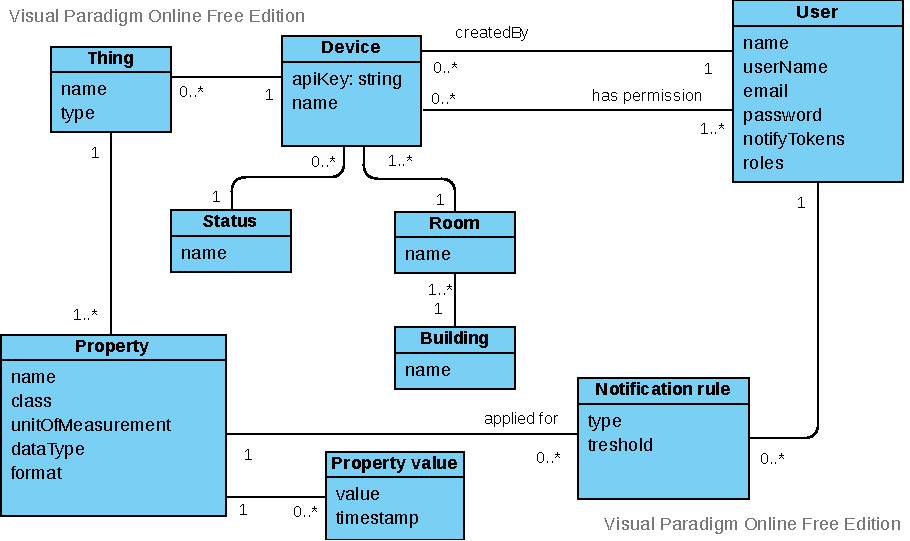
\includegraphics[width=\textwidth]{img/domain.pdf}
    \caption{  \label{domain-model}Doménový model}
\end{figure}
\begin{itemize}
    \item \textbf{Uživatel (User)} - osoba, která interaguje se systémem pomocí uživatelského rozhraní.
    \item \textbf{Zařízení (Device)} - fyzické zařízení, které komunikuje s Platformou a dále se děli na věci.
    \item \textbf{Stav (Status)} - v jakém stavu se zařízení nachází (např. odpojeno).
    \item \textbf{Věc (Thing)} - logické uskupení vlastností, např. meteostanice.
    \item \textbf{Vlastnost (Property)} - určitá veličina, jejíž hodnota se odesílá na Platformu (např. teplota), která případně umožňuje být Platformou změněna/nastavena.
    \item \textbf{Hodnota vlastnosti} - hodnota v určitém časovém okamžiku.
    \item \textbf{Budova (Building)} - místo, které se dále dělí na místnosti.,
    \item \textbf{Místnost (Room)} - uskupení více zařízení.
    \item \textbf{Notifikační pravidlo} - za jaké podmínky se má uživateli odeslat notifikace.
\end{itemize}


\subsection{Případy užití}
Tato kapitola popisuje identifikované případy užití, které současně slouží jako podklad funkčních požadavků kladených na řešení. Figurují v nich následující aktéři:
\begin{itemize}
    \item Neautorizovaný uživatel - představuje nepřihlášeného uživatele webového rozhraní.
    \item Uživatel - přihlášený uživatel webového rozhraní.
    \item Administrátor - autentizovaný uživatele s vyšším stupněm oprávnění.
    \item Zařízení - koncové zařízení komunikující s Platformou
\end{itemize}

\begin{figure}[htbp]
    \centering
    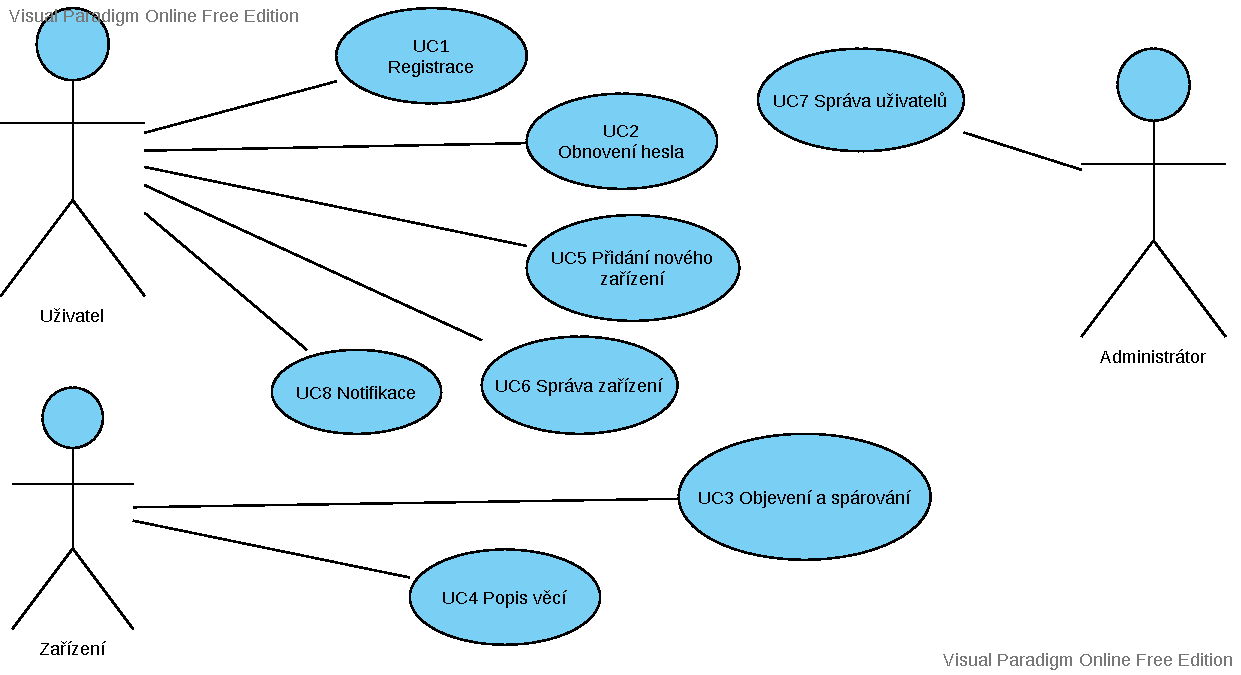
\includegraphics[width=0.9\textwidth]{img/use_case.pdf}
    \caption{Případy užití}
\end{figure}

\paragraph{UC1 Registrace uživatele}
Neautentizovaný uživatel vyplní registrační formulář obsahující jméno, přijmení, uživatelské jméno, heslo a email. Při zpracování požadavku na serveru bude zajištěna unikátnost uživatelského jména a emailu napříč databází. Uživatel bude informován o úspěchu/neúspěchu akce. Po úspěšné registraci bude automaticky přihlášen, pokud nezrušil ve formuláři zaškrtávátko \uv{Automaticky přihlásit}. Následně mu bude odeslán uvítací email na zadanou emailovou adresu.

\paragraph{UC2 Obnovení hesla}
Součástí přihlašovacího formuláře bude odkaz na stránku pro obnovení zapomenutého hesla, kde bude uživatel dotázán na emailovou adresu, kterou použil při registraci. Po zadání, pokud daná emailová adresa je součástí některého uživatelské účtu, bude odeslán email s odkazem pro obnovu hesla. Na tomto odkazu bude uživatel vyzván k zadání hesla nového.

\paragraph{UC3 Objevení a spárování nového zařízení}
Zařízení, pokud ještě není spárované s Platformou, po zapnutí vyzve uživatele k zadání svého uživ. jména k platformě. Toto zadání bude umožněno vytvořením Wifi přístupového bodu, na kterém poběží kaptivní portál - po připojení telefonem/počítačem se automaticky zobrazí webová stránka s formulářem pro zadání údajů. Následně se zařízení připojí k Platformě, ohlásí jaké má věci, popíše jejich vlastnosti, a bude ji informovat, kterému uživateli (podle zadaného uživ. jména) má zobrazit možnost přidání nového zařízení. Pokud si uživatel dané zařízení přidá (viz. \hyperref[UC5]{UC5}), Platforma následně odešle zařízení API klíč, které si ho uloží a přihlásí se pomocí toho klíče k Platformě (nyní je spárované).

\paragraph{UC4 Popis věcí}
Zařízení při ohlašování definice věcí a jejich vlastností musí oznámit mimo jiné typ věci. Platforma bude podporovat kromně generického (generic) typu další 3 typy věcí, pro které bude speciální zobrazení v uživatelském rozhraní:
\begin{itemize}
    \item \textbf{Switch} - přepínač, který se nachází ve stavu on/off. V rozhraní bude věc reprezentována dvoustavovým přepínačem, který při kliknutí odešle změnu o stavu na druhý, než ve kterém se aktuálně nachází. (využití např. vypínač světla)
    \item \textbf{Activator} - spínač, který má pouze jeden stav. V rozhraní bude věc reprezentována tlačítkem, které na stisk odešle aktivaci zařízení. (využití např. ovladač pojízdné brány)
    \item \textbf{Sensor} - v rozhraní bude reprezentován jako widget zobrazující aktuální hodnotu první vlastnosti. Po rozkliknutí se zobrazí graf vizualizující průběh hodnoty v čase za posledních 24h.
    \item \textbf{Generic} - obecný typ, u kterého zařízení popíše strukturu, datové typy a názvy příslušných vlastností. V uživatelském rozhraní bude věc reprezentována jako Widget, který po kliknutí zobrazí Dialogové okno umožňující zobrazení a ovládání všech vlastností dle konfigurace.
\end{itemize}

\paragraph{UC5 Přidání zařízení}
\label{UC5}
Uživateli na stránce \uv{Správa zařízení}, v případě že bude detekováno nové zařízení, v sekci \textit{Přidat zařízení} se zobrazí (bez nutnosti aktualizace stránky) možnost přidat nové zařízení. Při kliknutí na tlačítko přidat se zobrazí jednoduchý formulář pro zadání umístění a názvu zařízení - bude předvyplněn název, který ohlásilo zařízení. Uživatel formulář potvrdí, systém následně vytvoří dané zařízení, přidá uživateli k němu oprávnění a na stránce \uv{Ovládání} už bude uživatel moci sledovat aktuální stav věcí a případně je i ovládat (pokud to umožňují).

\paragraph{UC6 Oprávnění}
Uživatel na stránce \uv{Správa zařízení} v sekci \textit{Správa} bude mít zobrazena všechna zařízení, ke kterým má uživatel oprávnění. Rozhraní umožní pro každé zařízení, ke kterému má příslušné oprávnění editaci, jeho smazání a pomocí formuláře editaci - názvu, umístění a změnu oprávnění pro jednotlivé uživatele. Tyto oprávnění budou rozděleny na tři úrovně:
\begin{itemize}
    \item Čtení - uživatel může si zobrazit veškeré údaje o zařízení.
    \item Ovládání - uživatel může zařízení ovládat.
    \item Správa - uživatel může editovat veškeré informace o zařízení (včetně oprávnění).
\end{itemize}

\paragraph{UC7 Správa uživatelů}
Administrátor má k dispozici stránku \uv{Správa uživatelů}, kde se mu zobrazí seznam všech registrovaných uživatelů. Jednotlivé uživatele může smazat a pomocí formuláře editovat všechny jejich osobní údaje a změnit heslo pro přihlášení.

\paragraph{UC8 Notifikace}
Rozhraní umožní uživateli nastavit pravidlo pro libovolnou věc, při kterém se odešle Web Push notifikaci (technologie umožňující serveru odeslat upozornění do prohlížeče klienta \cite{web-push}) na jeho zařízení. Pro nastavení bude zobrazený formulář umožňující výběr z vlastností dané věci, po vybrání se zobrazí výběr akce, při jejímž splnění chce uživatel obdržet notifikaci (překročení hodnoty / vždy / hodnota bude rovna) a případné pole pro zadání limitní hodnoty. Dále půjde zobrazit rozšířené nastavení pro konkrétní notifikační pravidlo umožňující nastavení času a konkrétních dnů v týdnu, kdy bude pravidlo platné (ve výchozím stavu bude vždy). Těchto pravidel si bude moci nastavit libovolný počet pro každé zařízení, ke kterému má oprávnění pro čtení.



\subsection{Nefunkční požadavky}

\paragraph{N1 Řešení spustinelné na Linux systému}
Systém bude možno provozovat na Linuxovém serveru (Debian) a také na platformě Raspberry Pi (verze 3B+/4, OS Raspbian).

\paragraph{N2 Responzivní webové rozhraní}
Aplikace bude nabízet responzivní webové rozhraní přizpůsobené pro zobrazení na mobilních zařízeních i stolních počítačích. Uživatelské rozhraní bude kompatibilní s prohlížeči Mozilla Firefox verze 80, Chrome verze 80 a Safari na iOS. Dále bude implementovat tzv. PWA (Progresivní webová aplikace) - bude využívat cache pro statické soubory pro rychlé načítání, spustitelné offline a na zařízení Android půjde v aplikaci chrome přidat na plochu a následně vypadat jako nativní aplikace.

\paragraph{N3 Rozhraní realizováno jako SPA}
Single page application (SPA) je webová aplikace, která utilizuje JavaScript tak, aby při interakci v rámci aplikace se nemusela načítat celá stránka, ale pouze chytře překresluje potřebné části. Výsledkem je mnohem přijemnější uživatelský zážitek, než při čekání na stažení a překreslení celé stránku po kliknutí na odkaz.

\paragraph{N4 Validace}
Uživatel v průběhu vyplňování formulářů v rozhraní obdrží interaktivní zpětnou vazbu v případě zadání nevalidních údajů. Interaktivní zpětnou vazbou jsou myšleny následující scénáře při průchodu formuláře:
\begin{itemize}
    \item Zadání nové hodnoty a opuštění pole - bude provedena validace a v případě nevalidního vstupu, bude uživatel vizuálně  upozorněn.
    \item Editace již zadané hodnoty v poli - validace bude provedena po každé změně (stisknutí klávesy), uživatel bude vizuálně upozorněn v případě nevalidního vstupu.
\end{itemize}

\paragraph{N5 Koncová zařízení}
Bude specifikován protokol, pomocí kterého s platformou budou zařízení komunikovat včetně definování schématu komunikace. Platforma umožní připojení libovolného zařízení, pokud použije definovaný protokol a bude se řídit schématem pro komunikaci.

\paragraph{N6 Výkonnostní požadavky}
Systém bude stabilní a zvládne obsluhovat stovku zařízení, kde každé bude odesílat změnu stavu s periodicitou 30 vteřin. Při tomto dlouhodobém zatížení nebude docházet k pádům systému ani k výraznému zpoždění komunikace (RESTful požadavky pod 500 ms).

\paragraph{N7 Konfigurace systému}
Veškerá konfigurace týkající se externích služeb jako jméno a heslo do databáze, číslo portu pro komunikaci atd. bude konfigurovatelné pomocí promněných prostředí (env variables). Detailní popis promněných bude obsažen v instalační příručce.


\subsection{Vybrané technologie}
Tato sekce se věnuje výběru protokolu pro komunikaci se zařízeními a programovacího jazyka, ve kterém bude řešení implementováno včetně výběru příslušných knihoven.

\subsubsection{Komunikační protokol}
Komunikačních protokolů je velké množství a jeho výběr přímo závisí na použitém přenosovém médiu. Při použití specializovaných sítí jako LoRa nebo Zigbee, nemáme moc velkou flexibilitu ve výběru. Zařízení podporující tyto specializované sítě jsou poměrně drahá, ale umožňují běh na baterii. Zatímco využití Wifi sítě nám dává obrovskou flexibilitu ve výběru protokolů a zařízení podporující připojení k Wifi nebyly nikdo více cenově dostupné jako dnes. Primárně z finančních nároků a možnosti využití stávající Wifi infrastruktury v domácnosti jsem se rozhodl pro Wifi jako bezdrátové médium. Současně díky přímé podpoře IP protokolu nebudu muset vytvářet bridge mezi serverem a sítí se zařízeními jako např. při použití Bluetooth či LoRa.

Z protokolů pro komunikaci je dnes nejpoužívanější HTTP, který ale nativně nepodporuje obousměrnou komunikaci, kdy zařízení může poslat zprávu serveru a stejně tak server zprávu zařízení, kterou pro ovládání zařízení budu potřebovat. Z obousměrných protokolů se velmi osvědčil WebSocket, který lze velmi snadno kombinovat s HTTP. Jedná se o protokol postavený nad TCP, který naváže spojení a obě strany mohou posílat zprávy \cite{websocket}. Je to velmi pěkné řešení pro posílání zpráv, ale neumožňuje nativně systematickou filtraci nebo odběr pouze určitých zpráv a nepočítá s během na nespolhlivých zařízeních. Proto přímo pro IoT vznikl otevřený síťový protokol MQTT, kterým jsem si zvolil jako komunikační protokol, jehož specifikaci vydává nezisková organizace \textit{OASIS}. Využívá asynchroní vzor \textit{publish-subsribe} (v podstatě rozděluje akci na dvě událost - vytvoření akce a její obsluhu) a byl speciálně navržen pro potřeby běhu na jednoduchých embeded zařízení s minimálním datovým tokem. Podrobný přehled všech protokolů využívaný pro IoT viz. \cite{protocols}.

\begin{figure}[htbp]
    \centering
    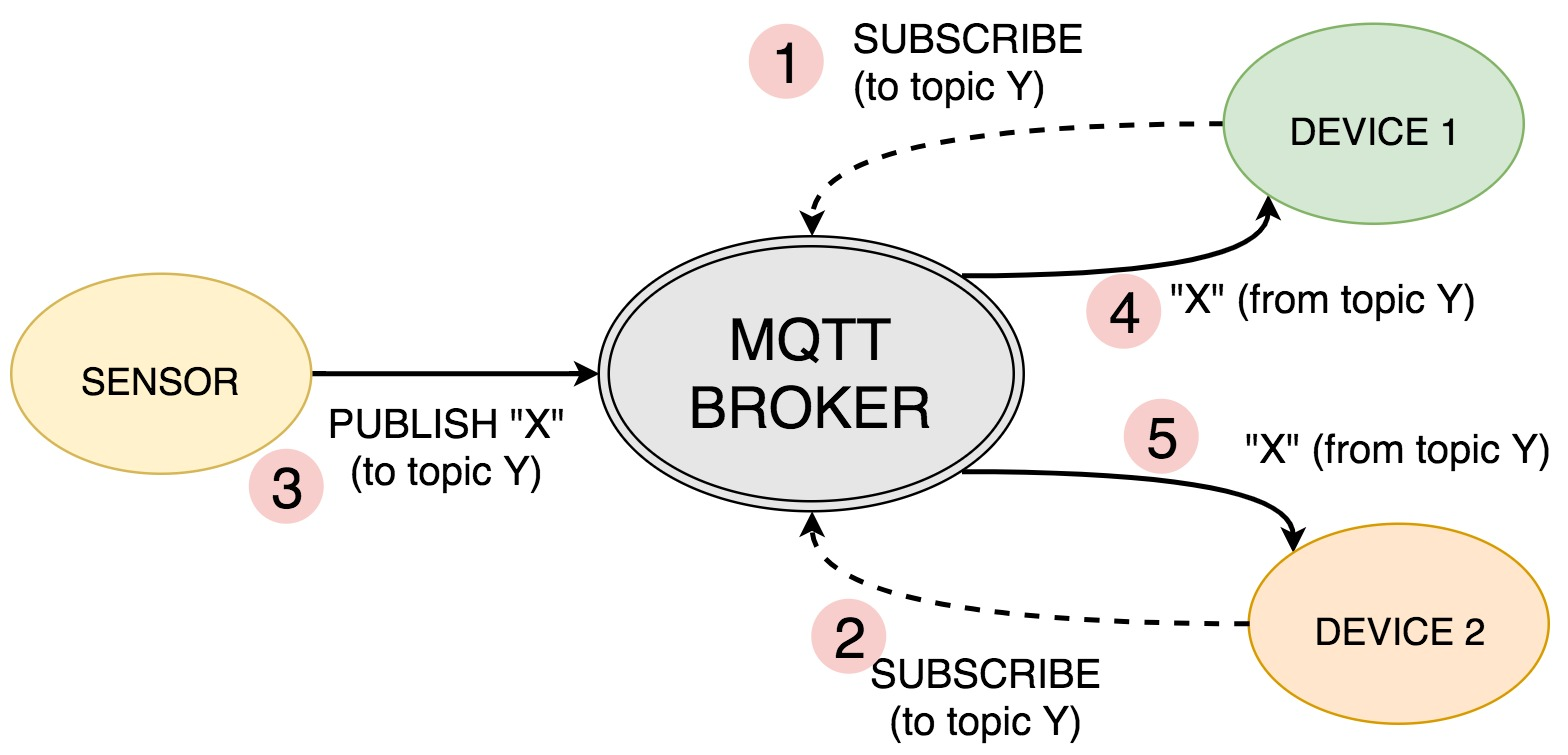
\includegraphics[width=0.7\textwidth]{img/mqtt-communication.jpeg}
    \caption{Ukázka komunikace MQTT \cite{img-mqtt-communication}}
\end{figure}

\label{mqtt-description}
MQTT se vyvýjí již od roku 1999 a momentálně nejpoužívanější verzí je 3.1.1, pro kterou vznikla specifikace v roce 2014. Protokol primárně běží nad TCP/IP, ale lze využít v jakékoliv síti, kde je zaručeno správné pořadí dat, beztrátovost a obousměrnost komunikace. Protokol definuje 2 typy entit: \uv{MQTT broker} a \uv{klient}. MQTT broker je server, který přijímá všechny zprávy od připojených klientů a přeposílá je příjemncům (klientům). MQTT klient je jakékoliv zařízení (od embeded až po server), které komunikuje s brokerem přes síť. \cite{mqtt}

Posílaná data jsou hierarchicky rozdělena do tzv. témat. Téma je textový řetězec o maximální délce 65\,536\,Bytů s oddělovačem lomítko (ukázka \uv{house/bedroom/light}). Pokud klient chce odeslat (publish) data, tak pošle zprávu brokeru s daty a tématem, do kterého zpráva patří. Broker potom zprávu odešle všem klientům, kteří jsou přihlášení k odběru (subscribe) z daného tématu. O odběr se klient musí přihlásit a to buď přímo specifikuje plný název topicu nebo částečný s použitím zástupných znaků. MQTT počítá s případnou nespolehlivostí koncových zařízení či sítě, a proto umožňuje klientovi při přihlášení definovat \uv{Last Will and Testament} (\hypertarget{LWT}{LWT}). Při přihlášení klient oznámí téma a zprávu, která se odešle v případě nesprávně odpojeného klienta (výpadek sítě / chyba zařízení). Takto lze notifikovat ostatní zařízení, že došlo ke ztráně spojení s daným klientem. \cite{mqtt}

Broker podporuje 3 třídy QoS (Quality of service), kterou lze specifikovat pro každou zprávu jednotlivě v závisloti na její důležitosti. Seřazeny jsou vzestupně dle náročnosti na systém (overhead) \cite{mqtt}:
\begin{itemize}
    \item \textbf{0 - Maximálně jednou} - zpráva je odeslána pouze jednou a klient ani broker nijak nepotvrzují její přjetí
    \item \textbf{1 - Alespoň jednou} - zpráva je odeslaná několikanásobně, dokud není potvrzené její přijetí
    \item \textbf{2 - Právě jednou} - odesílatel a příjemce navazují dvoucestný hand-shake, aby bylo zaručeno přijmutí zprávy právě jednou
\end{itemize}


\subsubsection{Programovací jazyk}
Programovacích jazyků je dnes na trhu dostupných stovky a každý má své specifické pozitivní i negativní vlastnosti. Při výběru je tedy vždy potřeba zohlednit jeho přínost pro použití na daném projektu. Kromě jazyka samotného je příhodné analyzovat dostupné knihovny a frameworky, které lze v projektu použít a značně tak urychlit celkový vývoj. Pro implementaci této práci byl zvolen jazyk JavaScript konkrétně jeho nadmnožina TypeScript a to z několika důvodů.

Vzhledem k povaze zvoleného protokolu pro komunikaci se zařízeními, jenž je založený na asynchronních zprávách, je JavaScript velmi vhodný, protože je založený na asynchronní event-driven \cite{nodejs} architektuře. Tato architektura nabízí velice elegantní přístup pro zpracování akcí, kde se musí čekat na výsledek jako např. u síťové komunikace či právě asynchronních zpráv. V tradičním jazyce jako Java nebo C++ se toto čekání musí řešit pracným vytvořením nového vlákna, které čeká na výsledek a následným zpracováním. V NodeJS je programátor od této problematiky odstíněn a může se tak plně věnovat tvorbě aplikační logiky, aniž by měl znalosti a zkušenosti s vícevláknovým programováním.

JavaScript je jediný programovací jazyk, který umožňuje psaní jak serverových aplikací, tak i uživatelského rozhraní formou webové stránky a jeho přímé vykonávání ve webovém prohlížeči klienta. Využití jednotného jazyka pro vývoj serveru i uživ. rozhraní přináší obrovskou výhodu v podobě možnosti sdílet nejenom definice pro objekty, ale i přímo části kódu. Toto je velmi vhodné například pro jednotné validace formulářů, různé datové transformace a sdílení aplikační logiky pro frontend \uv{optimistické aktualizace} (aktuální trend, nečekat na potvrzení požadavku ze serveru, ale rozhraní aktualizovat, jako by požadavek byl úspěšný a pouze v případě neúspěchu zobrazit stav ze serveru). Dále jednotný jazyk umožňuje programátorům při vývoji v případě potřeby pohodlně pracovat na obou částech aplikace, aniž by se museli učit nový jazyk.

\paragraph{TypeScript} Je nadmnožina JavaScriptu, která navíc přidává komplexní typový systém \cite{ts} a rozhodl jsem se ho využít jako hlavní programovací jazyk jak pro backend tak i frontend. Jedná se o OpenSource jazyk vyvíjený společností Microsoft, který jeho vznikem chtěl usnadnit přechod C\# a .NET vývojářům k webovým aplikacím \cite{ts}. Mnoho lidí z JavaScript komunity považuje TypeScript jako kontroverzní počin, protože přidává složitost k velmi elegantnímu jazyku a zvyšuje časovou náročnost vývoje. Já jsem dlouhou dobu tento názor také zastával, ale v posledních letech při práci na větších projektech a díky zkušeností z jiných jazyků (včetně striktně typových jako C++ a Java), jsem změnil svůj názor ve prospěch TypeScriptu. Souhlasím, že na první pohled prodlužuje dobu vývoje. Programátor musí psát věci navíc oproti čistému JavaScriptu, ale v dlouhodobém životním cyklu projektů se tato práce \uv{na víc} mnohonásobně vrátí. A to v podobě statické kontroly typů, která minimalizuje riziko pádu aplikace a umožňuje  lepší statickou analýzu kódu, a dále jako největší přínos pro mne jako programátora TypeScript přináší funkční \uv{našeptávání} ve vývojovém prostředí, které pro JavaScriptu i přes veškeré snahy bohužel funguje ve velmi omezené míře.

\subsubsection{Server}    %https://nodejs.org/en/docs/
%spousta jazyků, pro koncepsi asynchroních messages MQTT a Websocket se hodí NodeJS
Pro běh JavaScript na straně serveru existuje několik prostředí např. SpiderMonkey, NodeJS či Rhino. Pro realizaci bylo zvoleno prostředí NodeJS, které má pravděpodobně aktuálně největší a nejaktivější komunitu ze všech servrových prostředí pro běh aplikací napříč programovacími jazyky. Pro správu knihoven používá balíčkovací systém npm (jsou i jiné alternativy), ze kterého se stal největší ekosystém na světě, který je zastřešený neziskovou společností \uv{npm, Inc.} provozující centrální repozitář se všemi dostupnými moduly pro NodeJS. Díky sve centralizaci je velmi jednoduchý na používání, ale v posledních letech, kdy se JavaScript zpopularizoval a nyní je jedním z nejoblíbenějších jazyků \cite{survey-languages}, ukázala se centralizace jako poměrně nešťastné řešení kvůli vysokým nákladům na provoz infrastruktury. Pro představu velikosti ekosystému: npm v roce 2020 obsahoval 1\~200\~000 modulů a druhý největší systém RubyGems \uv{pouhých} 350\~000 \cite{modulecounts}. Všechny moduly jsou k dispozici zcela zdarma a díky takto aktivní komunitě lidí, kteří dávají k dispozici své knihovny ostatním, je vysoce pravděpodobné, že pokud chceme řešit nějaký problém, tak na něj již existuje knihovna.

%https://expressjs.com/
\paragraph{ExpressJS}\label{expressjs} Platforma bude implementovat RESTful webové rozhraní a pro jeho implementaci byl zvolen minimalistický framework ExpressJS. První jeho verze vznikla již v roce 2010 a do dnes je mezi vývojáři velmi oblíbený a v mnohém ovlivnil směr vývoje většiny frameworků. Jeho největší výhoda je vysoká flexibilita. Nabízí pouze základní definici způsobu pracování s HTTP požadavky a možnost registrovat tzv. middleware - software, který rozšiřuje funkcionalitu. Veškerá funkcionalita je dodávána pomocí middlewarů, které jsou k dispozici jako moduly. Vývojář si tedy může výsledný server poskládat přesně dle svých představ, kterých existují desítky vytvořených přímo od autorů a další stovky od komunity. \cite{expressjs}


\paragraph{AgendaJS} Knihovna pro perzistentní plánování úkolů pro NodeJS \cite{agendajs}. Umožňuje zpracování/plánování/perzistenci úkolů a jejich opětovné spouštění v případě chyby \cite{agendajs}. Tato knihovna bude primárně využita pro zajištění odeslání emailů a pro spouštění případných plánovaných akcí. Proč v souvislosti s odesláním emailů? Jejich zpracování je závislé na třetí straně - emailovém serveru, který nemusí být vždy dostupný. Pokud systém bude mět odeslat email, tak tímto způsobem bude zajištěno, že i v případě selhání bude email opětovně odeslán, jakmile to bude možné.

\paragraph{Socket.IO}\label{socketio} Pro zajištění aktualizace rozhraní v reálném čase bude využita knihovna SocketIO umožnující navázání obousměrného. Vyznačuje se vysokou spolehlivostí a rychlostí umožňující real-time komunikaci. Jedná se o velice populární a časem ověřené řešení, které zajišťuje kompatibilitu i s prohlížeči nepodporující moderní technologii WebSocket.


\subsubsection{Uživatelské rozhraní}
% React + Redux
Prvním bezesporu světoznámým průkopníkem ve světě JavaScriptu pro tvorbu uživatelského rozhraní byla knihovna \textit{jQuery}, která existuje dodnes, ale spíše se již považuje za přežitek doby. Dnes existuje obrovské množství Frameworků a knihoven pro tvorbu frontendu, ať pro tvorbu na straně serveru nebo přímo na straně uživatele v prohlížeči. Trend dnešní doby je přesouvat generování rozhraní na stranu uživatele, jak kvůli snížení výkonnostních nároků na server, tak spíše kvůli lepší odezvě a uživatelskému zážitku. Mezi nejznámější JavaScriptové frameworky patří bezpochyby Angular, Vue.js, Svelte a nesmím zapomenout na React, který je sice knihovna, ale řadí se na stejnou úroveň. Já jsem si zvolil jako hlavní prostředek pro tvorbu rozhraní React, právě proto že se jedná o knihovnu. Framework se vyznačuje tím, že vynucuje určité problémy řešit jistým způsobem bez možnosti volby. Má to své výhody a nevýhody a do větších týmů bych rozhodně volil raději framework. Tento projekt ale budu vytvářet primárně sám a mám velice rád flexibilitu a možnost volby. V začátcích to bývá časově náročnější, ale vidím v tom obrovskou možnost osobního růstu, protože při každé volbě musím hodnotit výhody/nevýhody a nakonec retrospektivně vidím následky svých rozhodnutí. Mimo to za vývojem Reactu stojí Facebook a je používán největšími technologickými spočnostmi světa (Yahoo!, Nextflix a Airbnb \cite{react-companies}), takže je jistá jeho dlouhodobá podpora a od roku 2013, kdy byla vydána první verze, je dobře odladěný a ověřený.

\paragraph{React} Je deklarativní, efektivní a flexibilní knihovna pro tvorbu rozhraní. Kód dělí do malých izolovaných částí kódu nazvaných \uv{komponenty}, které se skládají do sebe a mohou tvořit komplexní uživatelská rozhraní. Pro vysoký výkon využívá techniku virtuálního DOM - nejprve si vytvoří virtuální strom podoby rozhraní v paměti, který následně porovná s aktuální podobou vykreslenou v prohlížeči a zmanipuluje pouze ty části, které se od posledního vykreslení změnily. Díky tomu je velice efektivní a dokáže vykreslovat komplexní stránky s obrovským množstvím dat. \cite{react}

\chapter{Realizace}
Tato kapitola podrobně popisuje implementaci. Nejprve se věnuje popisu architektury serverové části a implementovaným bezpečnostním mechanizmům. Dále definicí MQTT schématu, který Platforma používá pro komunikaci se zařízeními, následované popisem implementace uživatelského rozhraní. Závěr kapitoly je věnován zamyšlení nad automatizací, nasazení celého řešení a tvorbě knihovny pro koncová zařízení a její následné demostraci při výrobě ukázkového zařízení.


\section{Serverová část}
% Popsat rozdělení na 2 BE servery, API rozhraní, komunikace webSocket -> ukázat sexy diagram, Agenda (recoverable jobs)
Tato sekse popisuje návrh a realizaci serverového řešení včetně architektury, implementovaných bezpečnostních mechanizmů a definicí schématu pro komunikaci s platformou na protokolu MQTT.


\subsection{Architektura}
Systém implementuje relaxovanou \textbf{Třívrstvou architekturu} obohacenou o vzor \textbf{Publish subscribe}. Základní myšlenkou Třívrstvé architektury je oddělení zodpovědnosti do tří vrstev, kde každá vrstva by měla být zodpovědná za určitou činnost a nepřesahovat svým rozsahem do zodpovědnosti jiné. Jednotlivé vrstvy:
\begin{itemize}
    \item Controller (řadič) - prostředník pro komunikaci mezi uživatelským rozhraním a služeb, které systém nabízí.
    \item Service (služba) - část systému obsahující aplikační logiku, jejímž úkolem je vykonání určitých úkolů (např. vytvoření uživatele).
    \item Data access layer (vrstva pro přístup k datům) - vrstva zapouzdřující přístup do databáze, která vytváří dle požadavků příslušné dotazy a výsledky mapuje na objekty, se kterými se pracuje lépe než s textovými záznamy.
\end{itemize}

Vzor \textbf{Publish subscribe} přidává navíc asynchronní zpracování událostí. Toto řešení je velmi užitečné v případě, pokud je potřeba navázat nějaké akce (nejčastěji volání třetí strany např. kvůli analytickým údajům). Například pokud vytvoříme řadič pro registraci uživatele, tak od něj očekáváme, že vytvoří uživatele a to je vše. Jsou ale situace kdy potřebujeme navázat další akce, které nemají žádnou přímou spojitost s danou odpovědností (např. zalogování do google Analytics nebo odeslání emailu). Přidáním této akce přímo do kontrolleru bychom porušili \textit{Princip jedné odpovědnosti} (Single-responsibility principle), který říká, že každý objekt (v tomto případě řadič) by měl vykonávat pouze činnost, která se od něj očekává. V tuto chvíli se hodí vzor \textit{Publish subscribe}, který umožní v řadiči vyslání (emit) události, že byl registrován uživatel a veškeré nesouvisející akce se vykonají v obsluze dané události v jiné části systému. Díky tomu nedojde k porušení Principu jedné odpovědnosti a kód řadiče dělá přesně to, co se od něj očekává a nic víc.

Servrová část je rozdělena na dva separátní procesy kvůli zvýšení odolnosti, aby v případě pádu jedné z části buď fungovalo uživatelské rozhraní nebo část obsluhující komunikaci se zařízeními.
\begin{itemize}
    \item \textbf{Backend} - dává k dispozici RESTful rozhraní pro kompletní ovládání Platformy, dále vykonává naplánová akce jako odesílání emailů.
    \item \textbf{Backend-mqtt} - interaguje se zařízeními přes MQTT broker a odesílá real-time změny na frontend.
\end{itemize}

\begin{figure}[htbp]
    \label{packages-uml}
    \centering
    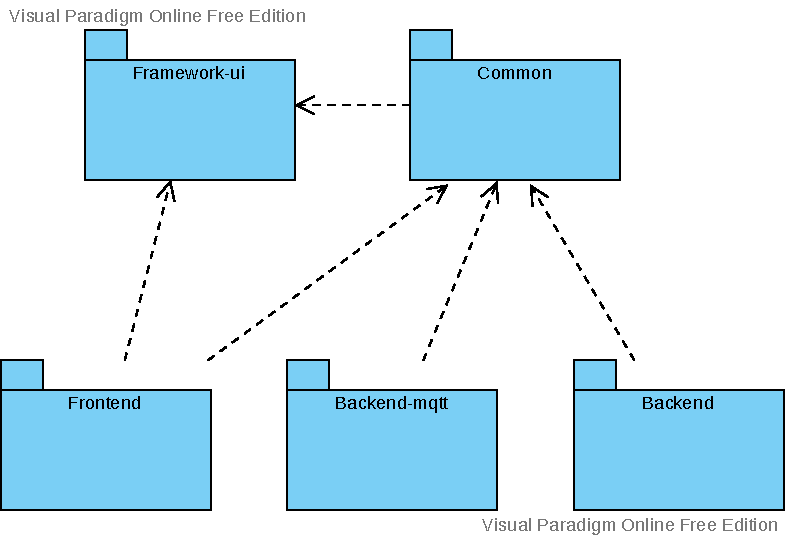
\includegraphics[width=0.5\textwidth]{img/packages.pdf}
    \caption{Diagram rozdělení balíčků}
\end{figure}

\subsection{Databáze}
Databáze je kritická část každého systému, protože se stará o perzistentní uchování dat, bez kterého bychom ztratili veškerá data při restartu či výpadku elektrické energie. Databáze lze obecně rozdělit do dvou skupin. První je označována jako SQL, která je založená na předpokladu, že objekty (reálného či virtuálního světa) lze přesně definovat a zpravidla mají mezi sebou vztah (relaci) např. potraviny a nákupní košík - vložení potravin do košíku lze reprezentovat vztahem, který je mezi danou potravinou a košíkem (je vložena / není). SQL databáze se orientují právě na zachycení vztahů mezi strukturovanými daty. Naopak druhá skupina NoSQL (Not only SQL) se orientuje na ukládání nerelačních nestrukturovaných dat. Problematika různých typů databází je velice rozsáhlá a více se jí zde věnovat nebudeme. Pro podrobnější popis doporučuji \cite{sql-and-nosql}.

Oba přístupy mají své výhody a nevýhody je potřeba volit databázi na základě druhu dat, která bude uchovávat. Pro mé řešení jsem zvolil NoSQL databázi z následujících důvodů. Vzájemná provázanost dat bude naprosto minimální viz. sekce s doménovým modelem \ref{domain-model}. Dále zařízení mohou produkovat potencionálně obrovské množství dat, pro což se NoSQL databáze hodí lépe, protože umožnují tzv. horizontální škálování (rozložení zátěže na více fyzických strojů), které pro SQL databáze lze efektivně využít pouze pro čtení nikoliv zápis. NoSQL databáze také umožňuje mnohem dynamičtější vývoj, protože SQL databáze vyžadují pevnou strukturu dat a i malá změna struktury znamená často velmi složitou migraci všech dat, zatímco NoSQL databáze umožňují ukládání dat bez nutnosti definovat jejich strukturu.

Specificky byla zvolena NoSQL databáze MongoDB, která je velmi populární mezi vývojáři, má skvělou podporu ze strany knihoven v NodeJS světě a pro uchovávání dat používá formát podobný formátu JSON (MongoDB nazývá formát BSON \cite{bson-vs-json}), což se velmi snadno kombinuje s jazykem JavaScript, který JSON používá pro nativní objekty.

\paragraph{Mongoose} je knihovna pro NodeJS, která vytváří nad MongoDB objektovou abstrakci a spoustu dalších užitečných funkcí jako validace a type cast \cite{mongoose}. Základním prvkem je definování schéma pro jednotlivé dokumenty, což může vypadat jako návrat do striktního schématu u SQL databází, ale zde je schéma definované pouze na úrovni Mongoose, tedy mnohem flexibilnější a méně restriktivní. MongoDB nabízí oficiální knihovnu pro přístup do databáze, ale preferuji Mongoose, protože díky definici schémat mám obecně větší kontrolu nad daty, která se dostanou do databáze a mají výbornou rozsáhlou dokumentaci.

\subsection{Souborová struktura}
Oba procesy jsou rozděleny do separátních balíčků \textit{backend} a \textit{backend-mqtt}, které na sobě nejsou nijak závislé a pro sdílení společných částí kódu, primárně databázových modelů, je využíván balíček \textbf{common}. Následující souborová struktura pro oba procesy vychází ze článku \cite[Bulletproof node.js project architecture]{bolletproof-architecture}, která se mi velmi osvědčila v jiných projektech.
\dirtree{%
    .1 packages.
    .2 backend\DTcomment{obsluha RESTful rozhraní a úkolů}.
    .3 src.
    .4 api\DTcomment{zdrojové kódy pro jednotlivé endpointy}.
    .5 device.
    .5 discovery.
    .5 user.
    .4 jobs\DTcomment{definice úkolů pro AgendaJS}.
    .4 loaders\DTcomment{rozdělený startovací proces do modulů}.
    .4 middleware\DTcomment{definice vlastních middleware}.
    .4 services\DTcomment{zdrojové kódy služeb}.
    .4 subscribers\DTcomment{obsluha akcí na asynchroní události}.
    .2 backend-mqtt\DTcomment{oblsuha MQTT a Socket.IO}.
    .3 src.
    .4 api.
    .5 auth\DTcomment{endpoint pro RabbitMQ autentifikaci}.
    .5 actions\DTcomment{endpoint pro interní komunikaci s Backend}.
    .4 services\DTcomment{zdrojové kódy služeb}.
    .5 firebase\DTcomment{odesílání notifikací}.
    .5 mqtt\DTcomment{napojení na MQTT broker a obsluhu zařízení}.
    .5 websocket\DTcomment{real-time komunikace pomocí Socket.IO}.
    .4 subscribers\DTcomment{definice akcí na asynchroní události}.
    .2 common\DTcomment{obsahuje sdílené části kódu}.
    .3 src.
    .4 config\DTcomment{konfigurace načtená z promněných prostředí}.
    .4 models\DTcomment{definice mongoose schémat a typů}.
    .4 utils.
}


\subsection{Proces Backend}
Tento proces s využitím frameworku \hyperref[expressjs]{ExpressJS} implementuje webový server nabízející RESTful rozhraní pro vytváření, editaci a mazání všech entit Platformy. Data se odesílají a konzumují ve formátu JSON. Proces dále implementuje odesílání emailů.

\subsubsection{Popis rozhraní}
Všechny endpointy, až na přihlášení a registraci uživatele, vyžadují autentizační token v hlavičce požadavku. Odpověď se potom liší podle oprávnění daného uživatele. Ukázka rozhraní:
\begin{itemize}
    \item POST /user - vytvoří nového uživatele
    \item GET /device - vrací seznam zařízení
    \item DELETE /device/:deviceId - odstraní dané zařízení
    \item PATCH /device/:deviceId - aktualizuje zařízení
    \item GET /device/:deviceId/thing/:thingId/history?from=\&to - vrací historická data pro specifikovanou věc, parametry specifikují časový rozsah
    \item PUT /device/:deviceId/thing/:thingId/notify - nastaví notifikační pravidla pro určitou věc
    \item PATCH /device/:deviceId/thing/:thingId - aktualizuje state pro danou věc
\end{itemize}

Server na požadavky odpovídá následujícími HTTP kódy (tělo odpovědi obsahuje podrobnější chybovou hlášku):
\begin{itemize}
    \item 200 - v pořádku, součástí těla odpovědi jsou data
    \item 204 - v pořádku, tělo odpovědi je prázdné
    \item 400 - chybný požadavek
    \item 403 - nedostatečné oprávnění
    \item 404 - požadovaný zdroj nebyl nalezen
    \item 500 - chyba serveru
\end{itemize}


\subsection{Proces Backend-mqtt}
Tento proces implementuje autentizační rozhraní, které používá MQTT broker pro autentifikaci jednotlivých zařízení. Je přihlášen k odběru všech zpráv z MQTT brokeru, na které příslušně reaguje - vytváří nově objevená zařízení, ukládá stav zařízení, změny stavu jejich vlastností a odesílá real-time změny na rozhraní pomocí knihovny Socket.IO. Dále implementuje RESTful rozhraní pro interní komunikaci s procesem Backend, které umožňuje nastavení změnu stavu vlastnosti a inicializaci párování nového zařízení. Toto rozhraní je z důvodu oddělení odpovědností, kdy tento proces řeší obsluhu zařízení přes MQTT, zatímco proces Backend výhradně komunikaci s uživatelským rozhraním.


\subsection{Bezpečnost}
Platforma zpracovává uživatelská data a proto je nutné tato data chránit (s ohledem na soukromí uživatelů a i z pohledu zákona). Následující text pojednává o implementovaných bezpečnostních prvcích.

RESTful rozhraní je přímo dostupné z internetu a proto je velice důležité ho správně zabezpečit proti zneužití. Proti velkému množství útoků se lze bránit správným nastavením HTTP hlaviček. Toto sice nechrání před přímými útoky, protože útočník může hlavičky ignorovat, ale chrání uživatele tak, že informují jejich prohlížeč o povoleném chování stránky např. odkud je bezpečné stahovat kód. Tímto způsobem lze primárně předejít útokům typu \textit{Cross-site scripting} (vložení/podstrčení cizího JavaScript kódu do stránky) a jiným druhům \textit{Cross-site infections} (vkládání html, stylů a jiných objektů) a \textit{Clickjacking} (překrývání klikacích prvků jinými s úmyslem propagace kliknutí na prvek, který chce útočník). Pro nastavní hlaviček jsem využil middleware \uv{helmet}, který je doporučený projektem OWASP (Open Web Application Project) \cite{owasp-cheatsheets}, který se přímo zabývá bezpečností webových aplikací. Pro ochranu přihlášení před útokem typu \textit{Brute-force} (hrubou silou) jsem použil middleware \uv{express-rate-limit} s omezením množství požadavků na jednu ip adresu za časový úsek. V případě potřeby je ale velmi snadno rozšiřitelný o komplexnější omezení (např. limit pokusů pro kombinaci uživatelského jména a ip adresy).

Pravděpodobně nejznámější typ útoku je \textit{SQL Injection}. Díky zvolení databáze typu NoSQL systém touto zranitelnosti netrpí přímo, ale jejím ekvivalentem v podobě \textit{NoSQL Injection}. Princip tohoto útoku je velmi jednoduchý. Zranitelnost vychází ze všech uživatelských vstupů, která se používají pro vytváření dotazů do databáze. Při sestavování těchto dotazů lze chytře využít možnost daného dialektu databázového jazyka a kompletně modifikovat jeho význam. Způsob ochrany spočívá v odstranění či nahrazení všech potencionálně zneužitelných znaků z uživatelstkého vstupu. Konkrétně jsem využil middleware \uv{express-mongo-sanitize}, který odstraní ze všech potencionálně zneužitelných pozic v datech všechny znaky \uv{\$} a \uv{.}, které lze v případě MongoDB využít právě pro \textit{NoSQL Injection}.

Do systému mohou přistupovat klienti pod různými uživatelskými účty, které mají různá oprávnění vázaná k určitým zařízením. Proto je nutné zamezit přístup pouze k takovým zdrojům serveru, ke kterým má daný přihlášený uživatal přístup. Jak vlastně server pozná, kdo inicioval daný požadavek? V případě nestavového protokolu HTTP, musí iniciátor přiložit ke každému požadavku token, kterým prokáže svoji totožnost. K tomuto účelu se nejčastěji využívaly dlouhé náhodné unikátní identifikátory, které byly uloženy v databázi u daného uživatele. Toto řešení ale vyžadovalo dotaz do databáze při každém požadavku pro ověření identity, což zbytečně zvyšuje zátěž na server. Proto byl vytvořen standard využívající asymetrickou kryptografii JWT (JSON Web Token, \cite[RFC 7519]{rfc-jwt}), který umožňuje aby po přihlášení server odeslal klientovi řetězec obsahující informace (např. id, jméno, příjmení, úrověň oprávnění) s cryptografickým podpisem a asymetrická kryptografie zaručuje, že nelze tyto informace modifikovat bez poškození integrity. Díky tomu odpadá nutnost pokaždé se dotazovat do databáze, protože stačí ověřit integritu tokenu. Tento postup má samozřejmě, ale i své negativní vlastnoti, kterými se zde však nebudeme zabývat. Pro detailnější vysvětlení doporučuji \cite{jwt-cons};

%https://news.netcraft.com/archives/category/web-server-survey/
Použití HTTPS (HTTP spolu se šifrováním SSL nebo TLS) je dnes samozřejmností v případě, že se na stránce zadávají jakékoli údaje. NodeJS přímo podporuje šifrované HTTP, ale správa certifikátu i nastavení není úplně přímočaré. Proto jsem NodeJS použil jako HTTP server s reverzním proxy serverem Nginx, který s klienty již komunikuje pomocí zabezpečeného spojení. Nginx je široce podporován různými nástroji pro správu webů mimo jiné nástrojem \uv{Certbot}, který umožňuje automatické získání bezplatného certifikátu nutného pro provoz HTTPS. Lze velmi snadno konfigurovat a nabízí pokročilé funkce jako \textit{load balancing}.

Veškerá komunikace mezi koncovými zařízeními a Platformou probíhá přes protokol MQTT a proto zabezpečení tohoto kanálu je nezbytné. Není žádoucí, aby třetí strana mohla posílat požadavky pro změnu stavu zařízením, i odposlouchávání zpráv je bezpečnostní riziko (z odposlechu pohybových čidel lze zjistit, zda je někdo doma, zlatý důl pro zloděje). Šifrování MQTT dokáže zajistit využitím protokolu nižší vrstvy TLS (označováno jako \textit{mqtts} nebo \textit{mqtt over tls}). Toto řešení zamezí odposlechnutí komunikace mezi Brokerem a zařízením. Většina existujících řešení pro domácnost další bezpečností prvky neimplementují a následkem toho sice nelze odposlechnout komunikace, ale lze se jednoduše přihlásit k Brokeru k odběru všech zpráv. Já však považuji toto řešení jako nedostatečné a proto implementuji systém pro autentizaci (ověření identity) i autorizaci (kontrola oprávnění pro přístup k danému zdroji). MQTT specifikace umožňuje přihlášení pomocí uživ. jména a hesla nebo certifikátu. Vzhledem k omezenému výpočetnímu výkonu ESP8266 jsem nucen využít kombinaci jména a hesla, protože rozumný výpočet asymetrických šifer je za hranicí jeho možností. Jako MQTT Broker využívám RabbitMQ, který podporuje definici vlastního backendu pro kontrolu oprávnění přes RESTful rozhraní. Toto řešení mi umožňuje kontrolovat přihlášení jednotlivých zařízení a i následně jednotlivé požadavky k publikaci a odběru zpráv. Součástí dat, které předává RabbitMQ autentizačnímu serveru je i název tématu do kterého chce zařízení zapisovat nebo z něho číst. Mohu tak přesně specifikovat, jestli danému zařízení bude umožněn přístup do daného tématu či nikoliv.

\subsection{Validace}
\label{BE:Validace}
% Vlastní framework, interaktivní validac na FE -> best UX, descriptory
Webové aplikace se stávají stále více komplexní se složitější datovou strukturou. Z pohledu systému je důležité validovat veškerá data, která přijdou od třetí strany před tím, než s nimi začneme pracovat, protože se nelze pouze spoléhat, že nám je někdo poslal ve správném formátu, v horším případě útočník bude záměrně posílat chybná data s nějakým postranním úmyslem. Dále z pohledu uživatele, je pro něj důležité, aby formulář byl intuitivní a na případné chybně zadané hodnoty byl ihned upozorněn - z vlastní zkušenosti vím, že není nic horšího než vyplnit dlouhý formulář, který se zdá naprosto validní, stisknout tlačítko odeslat a následně vidět nic neříkající hlášku \uv{Nevalidní formulář} bez jakýchkoliv upřesňujícíh informací.

%http://sumitshresthatech.blogspot.com/2012/03/field-and-field-descriptor-pattern.html
Využití stejného programovaícho jazyka jak na backendu, tak frontendu mi umožňuje využít stejný způsob validace dat na obou stranách, který poskytne uživateli okamžitou odezvu bez nutnosti duplikace validační logiky. Implementoval jsem si proto vlastní framework, který je založen na vzoru \uv{Field and Descriptor Field} \cite{field-descriptor-pattern}. Podle tohoto vzoru vstupují do systému dva separátní vstupy. Field obsahuje reálnou hodnotu pole a Deskriptor popisuje správný formát hodnoty pole. Systém při validaci určité hodnoty si nejprve načte příslušný deskriptor a následně aplikuje validační logiku dle konfigurace v deskriptoru na hodnotu.

Pomocí deskriptorů se definují struktury dat celých formulářů. Většina RESTful endpointů konzumuje v těle požadavku formulář, který je předem systémem zvalidován (pomocí middlewaru). Výstupem validace je seznam všech polí, která nejsou validní a chybové hlášky obsahující přesný popis, proč validace selhala.

\subsubsection{Field Deskriptor}
Deskriptor se definuje pro každé formulářové pole, společně tvořící deskriptor pro celý jeden formulář. Datovou strukturu reprezentující formulář lze libovolně zanořovat a struktura odpovídá 1:1 struktuře držící samotná formulářová data. Ukázka deskriptoru pro formulář obsahující jedno pole:

\begin{verbatim}
{
    FORM_NAME: {
        userName: {
            // sebereflektivní cesta k deskriptoru
            deepPath: "FORM_NAME.userName",        
            label: "Název který se zobrazí u pole v UI",
            // pokud vrátí false, tak required bude ingorováno
            when: (formData) => formData.selected === "user", 
            // povinost vyplnění pole 
            required: true/false,
            // seznam validací, kterými se má validovat hodnota
            validations: [
                validationFactory('isString', {min: 3, max: 10})
            ],   
        }
    }
}
\end{verbatim}


\subsection{MQTT schéma}
% popis Homie komunikace + vlastní modifikace, ukázka na diagramu
MQTT je zvolený komunikační protokol umožňující odesílání a přijímání asynchronních zpráv identifikovaných tématem (popsáno v \ref{mqtt-description}). Jedná se tedy o definici obecné komunikace a pro účely této Platformy je potřeba vytvořit specifikaci, podle které se budou jednotlivá zařízení řídit při odesílání zpráv. Tímto bude jasně zadefinované, jak Platforma bude reagovat na jednotlivé zprávy a půjde implementovat bezpečnostní mechanizmy.

První prototyp jsem založil na vlastní struktuře témat na MQTT protokolu, na kterém zařízení oznamovala v jakém stavu se nachází a naslouchala pro případné požadavky na změnu. Uživatel při vytváření zařízení musel nadefinovat veškeré jeho vlastnosti pomocí poměrně rozsáhlých formulářů, následně byl vygenerován api klíč, který bylo nutné zadat do zařízení pro jeho úspěšné přihlášení k platformě. Toto řešení se ukázalo jako nešťastné, protože uživatel pro přidání zařízení musel mít rozsáhlé znalosti dané problematiky a tento proces byl velice časově náročný. Proto jsem se rozhodl, že místo aby uživatel definoval ručně každé zařízení, zavedu automatickou detekci (auto discovery) nových zařízení, které budou sama propagovat Platformě jaké věci a vlastnosti podporují.

Po mnohých experimentech jsem nakonec své řešení založil na konvenci \textbf{Homie} \cite{homie} specifikující strukturu MQTT témat pro automatickou detekci, konfiguraci a používání zařízení. Tento základ jsem obohatil mimo jiné o výměnu párovacího klíče a z důvodu, že konvence počítá s globálním unikátním identifikátorem pro každé zařízení, tak jsem přidal navíc unikátní prefix pro MQTT téma, které označuji jako \uv{realm} - tento prefix je unikátní pro každého uživatele a všechny jeho zařízení komunikují v tomto realmu. Toto mi umožňilo přesunout restrikci identifikátoru z globální na úroveň uživatele a zároveň dává každému uživateli vlastní prefix témat pro jeho zařízení či jiné využití a pro monitoring komunikace mu stačí se přihlásit k odběru všech zpráv z daného tématu. Moje řešení neimplementuje kompletní konvenci, ale pouze následující část.

Základem \textit{Homie} konvence je, že každé zařízení obsahuje uzly (věci) a ty mají vlastnosti. Příklad - zařízení auto má věc motor, které má vlastnosti teplotu a tlak. Každé zařízení komunikuje v tématu obsahující nějaký prefix a v další úrovní tématu id daného zařízení (ukázka \uv{homie/esp-1919/}). Homie specifikuje základní atributy tématu, které se používají pro konfiguraci a začínají symbolem \uv{\$}:
\begin{itemize}
    \item \$name - člověkem čitelný název
    \item \$state - v jakém stavu se dané zařízení nachází
          \begin{itemize}
              \item  Init - zařízení je připojené, ale ještě není plně připraveno
              \item Ready - je připraveno a plně funkční
              \item Sleeping - zařízení je uspané a momentálně nekomunikuje
              \item  Alert - zařízení vyžaduje pozornost
              \item Disconnected - odpojeno
              \item Lost - ztráta spojení (zařízení je poviné toto zadefinovat jako \hyperlink{LWT}{Last Will Testament})
          \end{itemize}
    \item \$nodes - seznam id věcí, které zařízení obsahuje oddělené čárkou
\end{itemize}

Pro prefix tématu \uv{homie/deviceId/nodeId} lze odeslat následující atributy:
\begin{itemize}
    \item \$name - člověkem čitelný název věci
    \item \$type - typ věci
    \item \$properties - seznam id vlastností, které daná věc obsahuje oddělené čárkou
\end{itemize}

Pro prefix tématu \uv{homie/deviceId/nodeId/propertyId} lze odeslat atributy:
\begin{itemize}
    \item \$name - člověkem čitelný název vlastnosti
    \item \$datatype - datový typ hodnoty vlastnosti (string, float, integer, boolean, enum)
    \item \$unit - jednotka hodnoty vlastnosti [volitelný]
    \item \$format - specifikace omezení pro daný datový typ. Pro float, integer lze uvést rozsah hodnot ve formátu minimální a maximální hodnota oddělená dvojtečkou (např. \uv{10:20}). Pro enum se specifikuje výčet možných hodnot oddělených čárkou (např. \uv{red,blue,orange}) [volitelný]
    \item \$settable - informace zda lze hodnotu vlastnosti nastavit (true, false) [volitelný, výchozí false]
\end{itemize}


%\begin{verbatim}
%prefix/deviceId/$name   -> Název zařízení
%prefix/deviceId/$nodes  -> seznam nodeId
%prefix/deviceId/nodeId/$name    -> Název uzlu
%prefix/deviceId/nodeId/$type    ->
%prefix/deviceId/nodeId/$properties
%    -> seznam propertyId
%prefix/deviceId/nodeId/propertyId -> Aktuální hodnota
%prefix/deviceId/nodeId/propertyId/$name -> Název
%prefix/deviceId/nodeId/propertyId/$datatype -> Datový typ
%prefix/deviceId/nodeId/propertyId/$unit -> Jednotka hodnoty
%prefix/deviceId/nodeId/propertyId/$settable
%    -> Lze/nelze nastavit vlastnost
%prefix/deviceId/nodeId/propertyId/set
%    -> Zařízení naslouchá pro změny pokud je settable
%\end{verbatim}

\subsubsection{Upravená specifikace}
Rozdíl v mém řešení oproti \uv{Homie} konvenci primárně spočívá v použití dvou rozdílným prefixů témat v závislosti, jestli zařízení již bylo spárováno (uživatel si dané zařízení přidal) či nikoliv. Toto opatření je z důvodu vyšší bezpečnosti, abych mohl oddělit již spárovaná zařízení od ostatních. Při prvním připojení se zařízení ohlásí v prefixu \uv{prefix/} následovaný identifikátorem zařízení stejně jako v případě \textit{homie} konvence. Oznámí svůj status, název a všechny své schopnosti (věci a vlastnosti). Toto téma je veřejně přístupné pro všechny zařízení, která se k MQTT brokeru přihlásí uživatelským jménem shodujícím se s identifikátorem zařízení na rozdíl od druhého prefixu \uv{v2/{realm}}, který je přístupný pouze zařízení, která se přihlásí pomocí platného api klíče s přístupem do daného realmu. Přidané atributy:
\begin{itemize}
    \item \$realm - do kterého realmu zařízení chce patřit (uživ. jméno uživatele)
    \item \$config/apiKey/set - tento atribut využívá Platforma pro odeslání api klíče. Zařízení je zodpovědně za přihlášení odběřu daného tématu.
    \item \$cmd/set - využívá Platforma pro odeslání příkazů, jmenovitě restart a reset.
\end{itemize}

Restrikce na typ věci:
\begin{itemize}
    \item sensor - senzor vyžadující mít první vlastnost číselného typu
    \item switch - přepínač vyžadující mít první vlastnost datového typu boolean
    \item activator - tlačítko vyžadující mít první vlastnost datového typu enum s jednou hodnotou
    \item generic - obecný typ
\end{itemize}

Přidán atribut pro téma definující vlastnosti:
\begin{itemize}
    \item \$class - do jaké třídy hodnota vlastnosti patří, možnosti: humidity, temperature, voltage, pressure. Tato hodnota ovlivňuje pouze uživatelské rozhraní, specificky jaká ikonka se u hodnoty zobrazí. [volitelné]
\end{itemize}


Následuje ukázka komunikace automatické detekce zařízení umožňující zapnutí/vypnutí světla, měření teploty s identifikátorem \uv{light} a hlásící se k uživateli s uživ. jménem \uv{pepa}:
\begin{verbatim}
prefix/light/$status   -> init
prefix/light/$name   -> Světlo
prefix/light/$nodes  -> sensor,switch
prefix/light/$realm  -> pepa
prefix/light/sensor/$name    -> Senzor
prefix/light/sensor/$type    -> sensor
prefix/light/sensor/$properties -> temperature
prefix/light/sensor/temperature/$name -> Teplota
prefix/light/sensor/temperature/$datatype -> float
prefix/light/sensor/temperature/$unit -> °C
prefix/light/sensor/temperature/$class -> temperature
prefix/light/switch/$name   -> Lustr
prefix/light/switch/$type   -> switch
prefix/light/sensor/$properties -> power
prefix/light/sensor/power/$name -> Lustr
prefix/light/sensor/power/$datatype -> boolean
prefix/light/$status    -> ready
\end{verbatim}

Pokud se detekované zařízení nachází ve stavu \uv{ready}, tak je zobrazeno příslušnému uživateli pro přidání. Pokud si ho uživatel přidá, tak Platforma odešle api klíč danému zařízení, který jeho přijetí potvrdí, klíč si uloží a následně se přepne do prefixu témat \uv{v2/{realm}/}. Pokračování ukázky:

\begin{verbatim}
prefix/light/$apiKey/set
    -> XXXXXXXXXXXXXXXX (odesláno Platformou)

prefix/light/$status    -> paired
v2/pepa/light/$status   -> ready

v2/pepa/light/sensor/temperature   -> 20.05
v2/pepa/light/switch/power         -> true
\end{verbatim}

\begin{figure}[htbp]
    \centering
    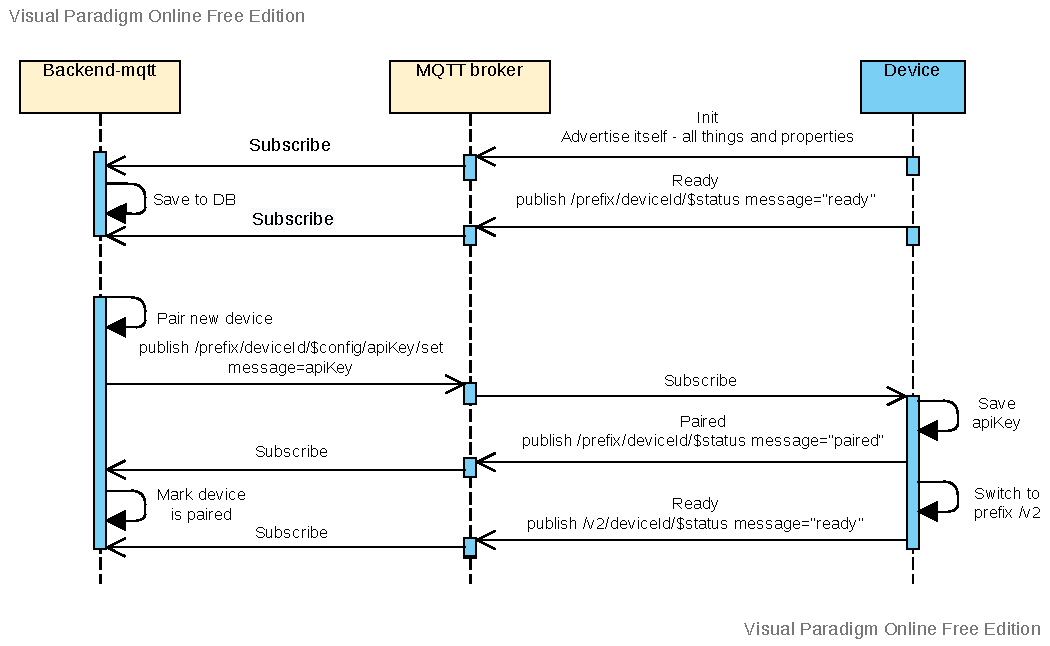
\includegraphics[width=\textwidth]{img/communication_part1.pdf}
    \caption{Diagram spárování zařízení}
\end{figure}



\section{Uživatelské rozhraní}
% Popis PWA, SPA, struktura složek, webSocket, no cookie (local storage)
Tato sekce se zabývá architekturou a implementací uživatelského rozhraní formou webové stránky. Implementace je rozdělena do dvou balíčků:
\begin{itemize}
    \item Framework-ui - obsahuje komplexní řešení pro validace formulářů včetně integrace s Redux (napojení na state, definice akcí a reducerů), implementuje znovu použitelné React komponenty, včetně komponenty řešící přímé napojení formulářového pole na state a obsluhu jeho validací (FieldConnector). Dále jazykovou lokalizaci pro systémové hlášky a nádstavbu nad fetch (api pro odesílání HTTP požadavků), která řeší zobrazení chybových hlášek a definuje flexibilnější rozhraní.
    \item Frontend - implementace samotné aplikace
\end{itemize}

\subsection{Frontend}
Uživatelské rozhraní je realizováno jako SPA - průchod celou aplikací je plynulý a nikdy nedochází k přenačítání celé stránky, ale pouze k překreslení potřebných částí. Toto řešení zlepšuje uživatelský zážitek, protože stránka zůstává pořád plně aktivní a při čekání na vyřízení požadavku uživatel může pokračovat v interakci. Také je zde implementován standard PWA - v podporovaných systémech jako je např. android lze aplikaci tzv. \uv{Přidat na plochu}, potom při otevření vypadá jako nativní aplikace (nemá zobrazený url bar). Statické soubory jsou v cache, díky čemuž je minimalizován datový přenost a stav aplikace je perzistentně ukládán, takže při zavření aplikace a následném otevření je stav plně obnoven a uživatel pokračuje přesně tam kde skončil naposledy a to i v případě bez přístupu k internetu - aplikace je kompletně načtena, ale následná interakce je již závislá na komunikaci se serverem.

\subsubsection{State management}
React je postavený na předávání dat mezi jednotlivými komponenty, které tvoří stromovou strukturu, data lze však předávat primárně z vrchu dolů a proto je poměrně složité ze spodní komponenty předat změnu do vrchní. Navíc dnešní aplikace pracují s obrovským množstvím dat, ke kterým potřebují přistupovat různé části aplikace a ideálně transparentní cestou data modifikovat a o této modifikaci se musí dozvědět všechny komponenty pracující s danými daty, aby dostali jejich aktuální verzi. Dnes již React obsahuje obecné řešení pro předávání dat, ale já jsem se rozhodl pro využití komplexního řešení s centrálním úložištěm stavu aplikace v podobě knihovny Redux, které nabízí více funkcí a je odzkoušené časem. Redux je založený na \uv{Observer pattern}. Tento návrhový vzor definuje dvě entity - předplatitel (pozorovatel) a vydavatel (pozorovaný). V praxi se jednotlivé komponenty přihlásí k odběru určitých dat (\uv{předplatí si je}) a v případě, že někdo chce data modifikovat, tak se stane vydavatelem a řekne, co modifikuje a jak vypadají nová data. Redux zajistí, že všichni předplatitelé dat, kterých se modifikace týka, dostanou jejich nejnovější verzi. V Reduxu se používá následující terminologie:
\begin{itemize}
    \item store - centrální úložiště dat (tvz. \uv{jediný zdroj pravdy})
    \item akce - popis k jaké změně dojde
    \item dispatch akce - odeslání určité akce k vykonání
    \item reducer - reaguje na odeslanou akci, obsahuje logiky pro modifikaci dat
\end{itemize}
\begin{figure}[htbp]
    \centering
    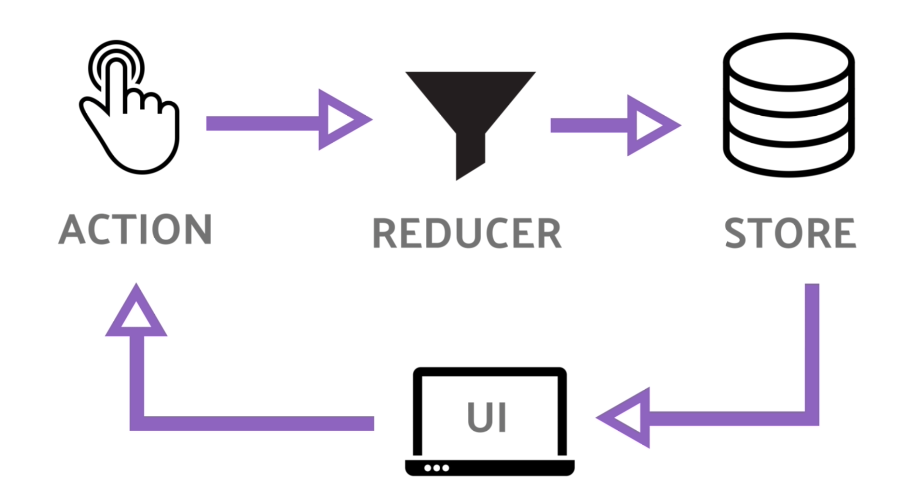
\includegraphics[width=0.5\textwidth]{img/redux.png}
    \caption{Redux tok dat \cite{img-redux-flow}}
\end{figure}

\subsubsection{Vzhled}
V kombinaci s Reactem jsem použil knihovnu Material-ui, která obsahuje velké množství nastylovaných komponent a komplexní řešení pro stylování React komponent. Tuto knihovnu používám již od prvopočátku jejího vzniku a velmi jsem si ji oblíbil kvůli detailní dokumentaci. Obsahuje vestavěné řešení pro \textbf{CSS-in-JS}, které mi jako programátorovi velmi vyhovuje, protože překlenuje spoustu limitací přímého použití CSS. Umožňuje definovat vzhled ve stejném souboru i jazyce jako samotnou React komponentu, díky tomu nemusí programátor přepínat kontext mezi různými jazyky a může se plně soustředit na vývoj uživatelského rozhraní.

\subsection{Souborová struktura}
\dirtree{%
    .1 packages.
    .2 framework-ui.
    .3 src.
    .4 api\DTcomment{implementace rozhraní pro odesílání požadavků}.
    .4 Components\DTcomment{React komponenty}.
    .4 localization\DTcomment{řešení pro lokalizaci systémových hlášek}.
    .4 privileges\DTcomment{pomocné funkce pro oprávnění a jejich dědičnost}.
    .4 redux\DTcomment{implementace akci a reducerů, primárně pro správu formulářových dat}.
    .4 validations\DTcomment{implementace validací}.
    .2 frontend.
    .3 public.
    .3 src.
    .4 Pages\DTcomment{jednotlivé stránky rozhraní}.
    .4 api\DTcomment{definice RESTful volání}.
    .4 components\DTcomment{sdílené komponenty napříč stránkami}.
    .4 containers\DTcomment{React kontejnery obalující celou aplikaci}.
    .4 firebase\DTcomment{služba pro registraci a obsluhu notifikací}.
    .4 store\DTcomment{inicializace Redux, definice akcí a reducerů}.
    .4 webSocket\DTcomment{služba pro inicializaci Socket.IO}.
}

\subsection{Validace}
Obecný princip fungování validací je popsán v sekci \hyperref[BE:Validace]{Backend}. Na Frontendu se validace používají pro upozornění uživatele na případně chybně zadanou hodnotu. Samotná formulářová data jsou spravována knihovnou redux, stejně jako celý state aplikace. Jejich struktura je shodná s deskriptory formuláře - deepPath se využívá pro získání příslušné hodnoty.

Pro vykreslení formulářového pole jsem připravil komponentu \textit{FielConnector}, které se předá typ pole (text, email, select atd.) a deepPath, podle které si nalezne příslušný deskriptor, ze kterého získá potřebné atributy a validace, které se provolávají v následujících případech:
\begin{itemize}
    \item uživatel poprvé zadává hodnotu a vyklikne (událost \uv{onBlur});
    \item uživatel edituje již zadanou hodnotu, potom se validace spouští po každé změně (událost \uv{onChange}).
\end{itemize}

\subsection{Rozhraní}
% TODO jaké obrazovky tam jsou, ukázka z rozhraní
Aplikace nabízí jednoduché uživatelské rozhraní s jedním menu pro navigaci mezi jednotlivými stránkami a tlačítko pro přihlášení, které otevře přihlašovací dialog.

Nepřihlášenému uživateli je k dispozici stránka pro registraci obsahující formulář. Po registraci je automaticky přihlášen a má k dispozici stránku pro správu zařízení a stránku pro ovládání a sledování jednotlivých věcí. Správa zařízení je rozdělena na dvě sekce, první obsahuje tabulku s detekovanými zařízeními, které lze přidat na dvě kliknutí. Druhá část obsahuje tabulku se zařízeními, ke kterým má uživatel oprávnění pro čtení a v případě oprávnění pro zápis, může editovat jejich informace, měnit oprávnění pro jednotlivé uživatele, odeslat příkaz pro restart nebo zařízení odstranit.

\begin{figure}[htbp]
    \centering
    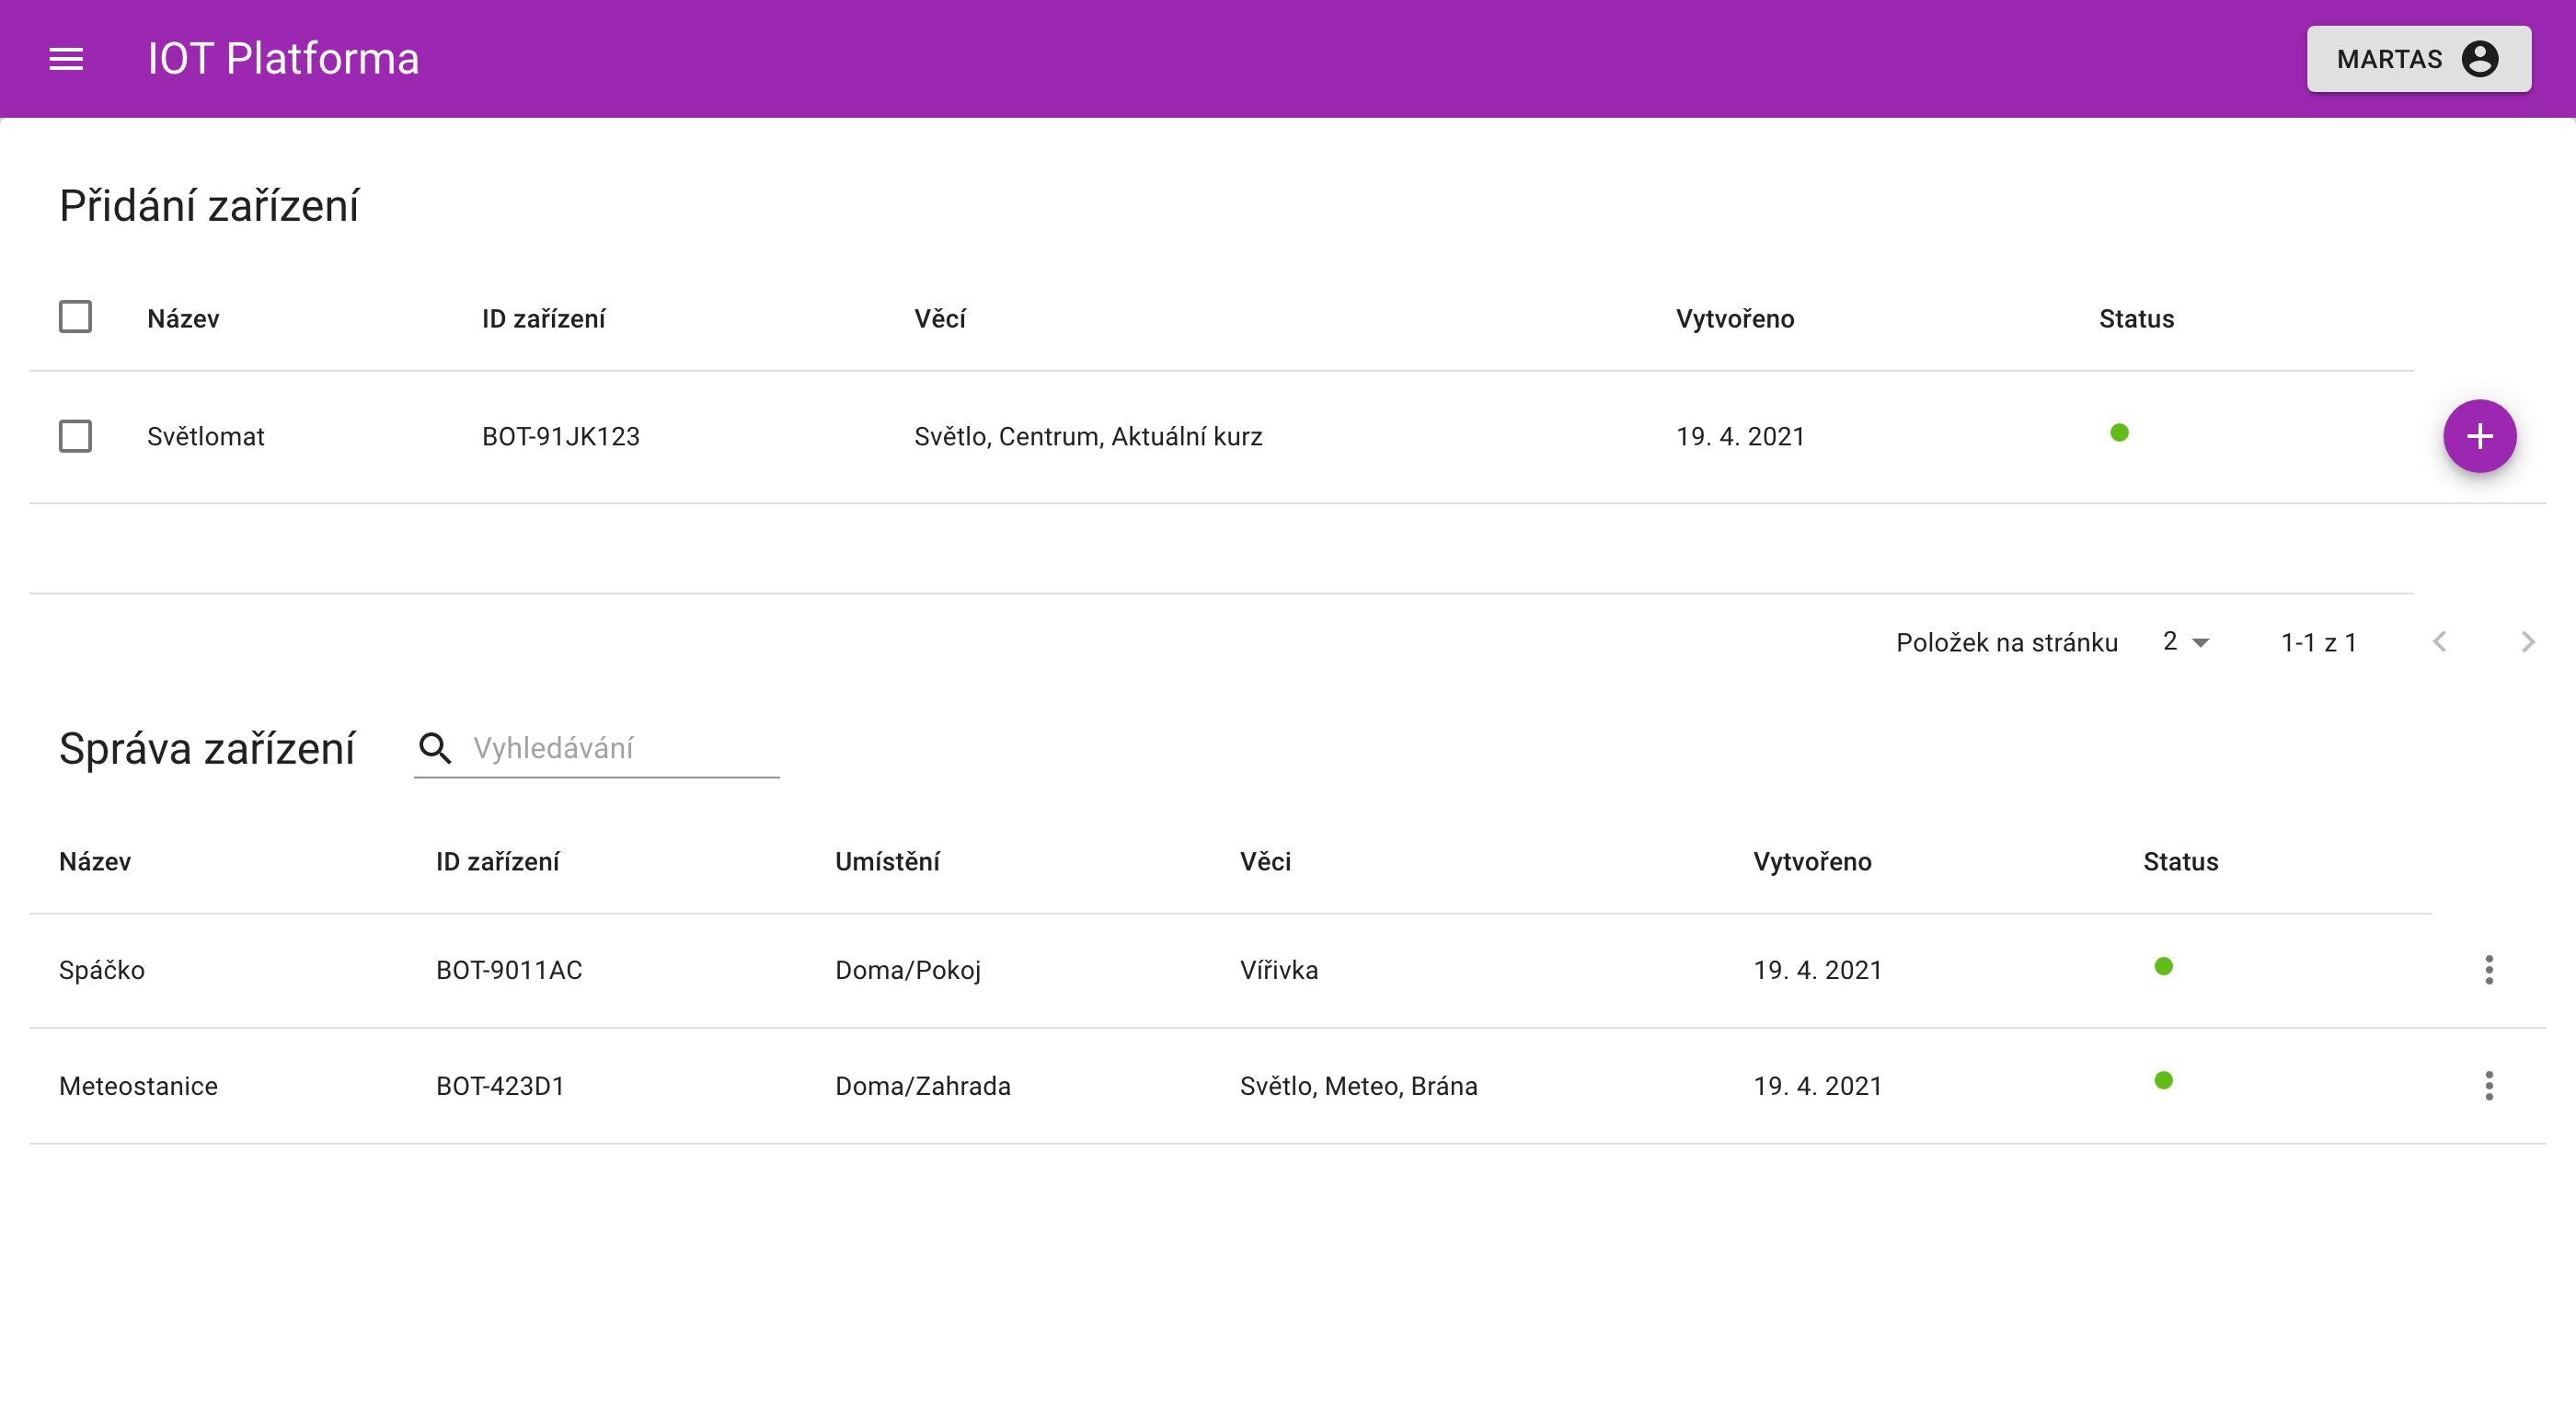
\includegraphics[width=\textwidth]{img/screens/deviceManagement2.png}
    \caption{Ukázka rozhraní - správa zařízení}
\end{figure}

Stránka pro ovládání zobrazuje widgety pro jednotlivé místnosti seskupené podle budov. Pokud místnost obsahuje nějakou věc typu senzor, tak aktuální hodnota je zobrazena na tomto widgetu. Po rozkliknutí místnosti jsou rozbrazeny všechny věci, která daná místnost obsahuje. S některými věcmi lze přímo interagovat (přepínač a aktivátor) a u senzoru je zobrazena aktuální hodnota. Pokud se dané zařízení nenachází v připraveném stavu, tak je uživatel upozorněn barevným kolečkem. Po kliknutí na název věci je zobrazeno dialogové okno, které se částečně liší v závislosti na typu věci:
\begin{itemize}
    \item \textbf{Generic} zobrazí aktuální hodnoty vlastností a je umožněna případná interakce s nimi.
    \item \textbf{Sensor} zobrazí stejný obsah jako pro \textit{generic} a navíc na začátku vykreslený graf vizualizující průběh hodnoty v čase za posledních 24 hodin.
    \item \textbf{Switch} zobrazí stejný obsah jako pro \textit{generic} a navíc časovou osu vizualizující aktivitu vlastnosti.
\end{itemize}

\begin{figure}
    \centering
    \begin{subfigure}{.5\textwidth}
        \centering
        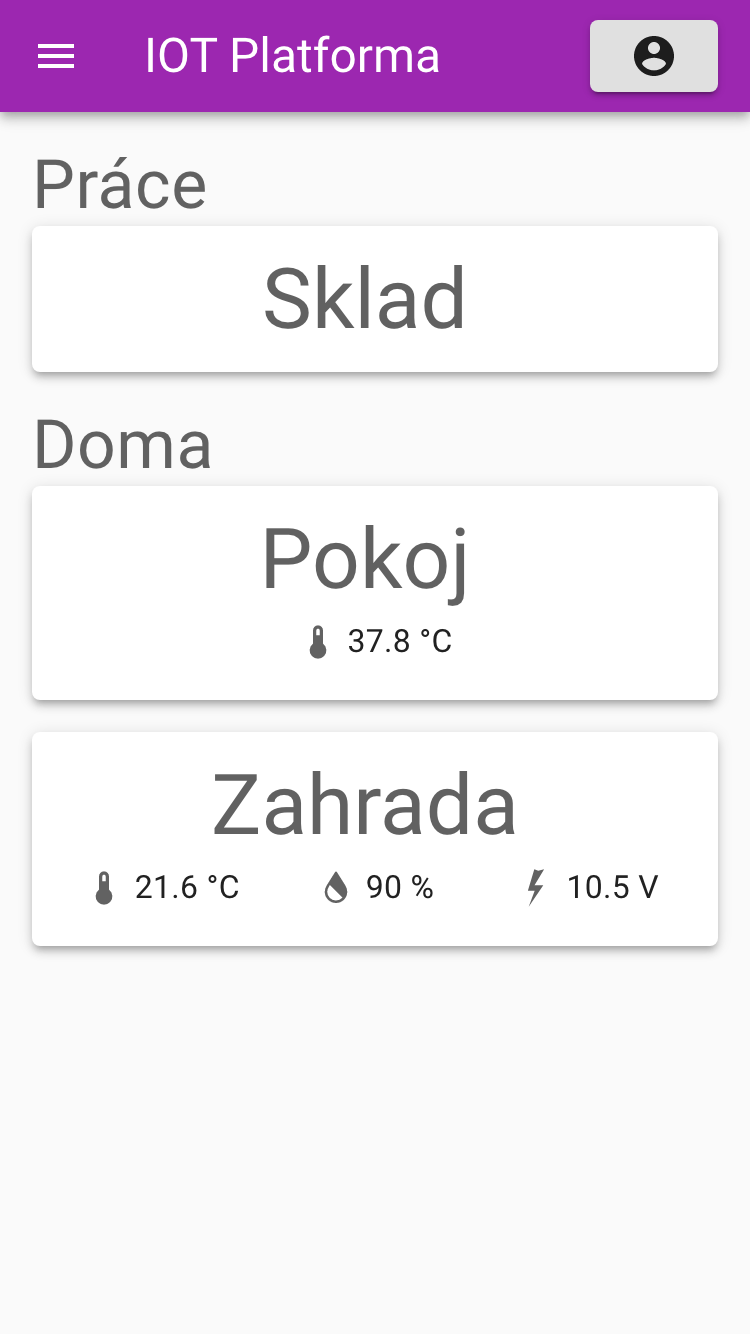
\includegraphics[width=.5\linewidth]{img/screens/buildings.png}
        \caption{Zobrazení místností}
        \label{fig:sub1}
    \end{subfigure}%
    \begin{subfigure}{.5\textwidth}
        \centering
        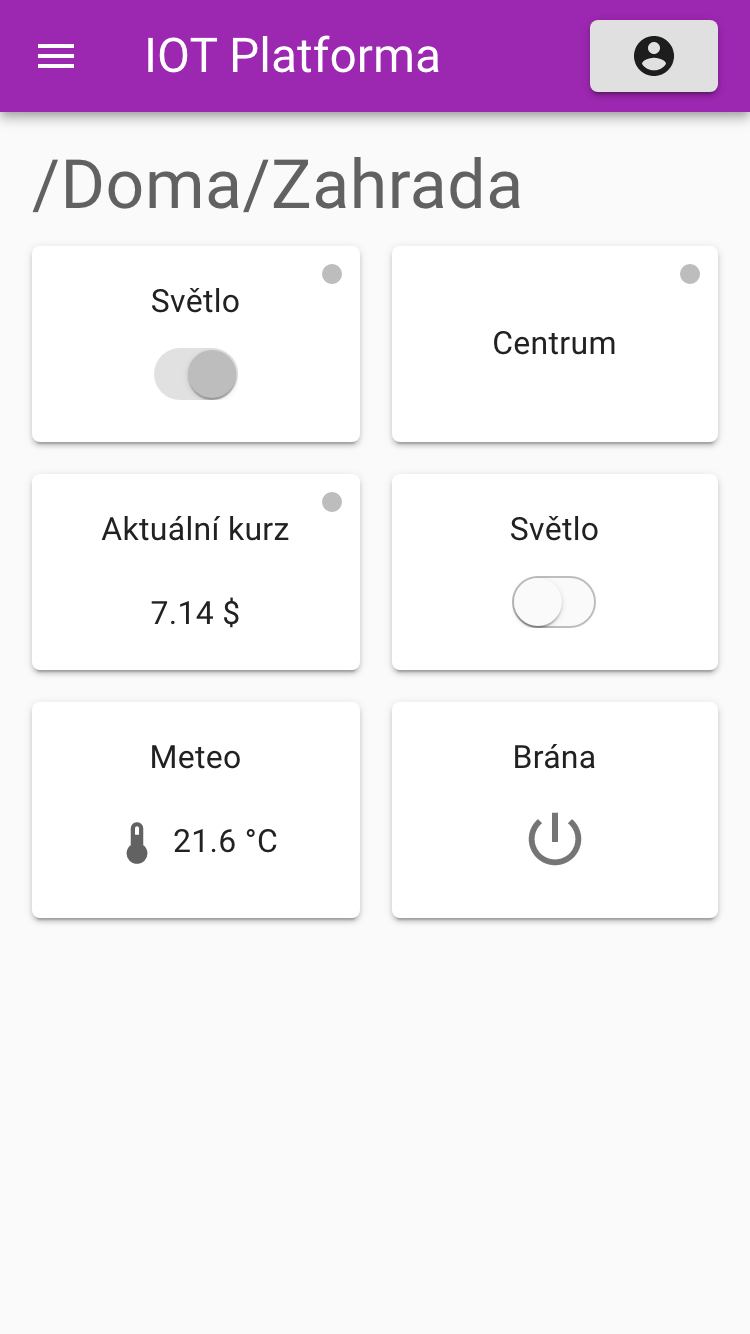
\includegraphics[width=.5\linewidth]{img/screens/room.png}
        \caption{Zobrazení místnosti}
        \label{fig:sub2}
    \end{subfigure}
    \caption{Ukázka rozhraní - výpis místností a jednotlivých věcí v místnosti}
    \label{fig:test}
\end{figure}

Přihlášený uživatel má dále k dispozici menu s možností editace vlastního uživatelskéhoo účtu a odhlášení.

Pokud má uživatel admninistrátorské oprávnění, tak má navíc k dispozici stránku pro správu uživatelů, ve které je tabulka zobrazující všechny uživatele s možností jejich editace a odstranění.



\section{Automatizace a hlasové ovládání}
Implementované řešení umožňuje automatizaci ze strany zařízení, která se mohou přihlásit k odběru zpráv z ostatních zařízení a příslušně reagovat. Možnost flexibilní automatizace ze strany Platformy vyžaduje nasazení velmi komplexního řešení, které z důvodu náročnosti nebylo implementováno. Nabízí se však využití nástroje \textbf{Node-Red}, který umožňuje vytvářet rozsáhlé datové toky pomocí vizuálního programování \cite{node-red}. Obsahuje intuitivní grafický nástroj pro vytváření složitých podmínek a následných akcí.

\begin{figure}[htbp]
    \centering
    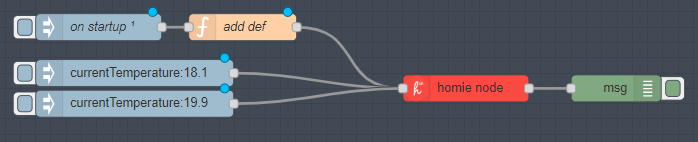
\includegraphics[width=0.9\textwidth]{img/homie-node-node.png}
    \caption{Node-Red ukázka definice akce \cite{node-red-homie}}
\end{figure}

Momentální řešení uživatelům umožňuje napojení vlastního nástroje, který bude přihlášen k odběru MQTT zpráv z jejich zařízení a mohou si tedy vytvářet datové toky v něm. Pro integrování řešení přímo do Platformy by bylo nutné analyzovat možnost použití Node-Red v tomto více uživatelském prostředí. Současně s tímto řešením by šlo podmiňovat notifikace složitějšími výrazy než pouze v závislosti na aktuální hodnotě dané vlastnosti, ale i v závislosti na jiných složitějších podmínkách.

Pro využití hlasového ovládání pomocí současných asistentek jako \textit{Siri} nebo \textit{Google Assistent} by bylo potřeba doimplementovat možnost vytváření tokenů pro přístup k API rozhraní pro jednotlivé uživatele a jejich správou. Následně by bylo možné využít v asistentkách možnosti definovat akci na hlasový povel, která by odeslala zadefinovaný požadavek na změnu jehož součástí by byl přístupový token pro autorizaci. Takto by bylo možné realizovat jednoduché povely pro změnu jedné vlastnosti. Pro definici složitější akce na hlasový povel by bylo možné využít webovou službu \textbf{IFTTT} \cite{ifttt} v kombinaci s asistentkou, která umožňuje vytvářet podmíněné příkazy a obsahuje integraci s velkým množství služeb třetích stran.


\section{Nasazení}
Celé řešení jsem nasadil na Linuxový server s operačním systémem Debian. Pro zjednodušení jsem se rozhodl celý proces automatizovat. Využil jsem OpenSource automatizační nástroj \textbf{Jenkins} \cite{jenkins}, který umožňuje psaní skriptů, které automaticky spouští při změně kódu (pro jeho verzování jsem využil nástroj GIT). Toto řešení mi umožňilo plně automatizovat sestavení celé aplikace a její následné nasazení na server pouhým uložení nové verze kódu. V případě výskytu chyby při sestavování jsem na ni byl ihned upozorněn a mohl ji opravit. Důvod využití právně nástroje Jenkins oproti alternativám např. \textit{GitLab CI/CD} či \textit{CruiseControl} spočívá v možnosti provozování nástroje zcela zdarma na vlastní infrastruktuře a také kvůli rozsáhlému systému pluginů, kterých má velký výběr na rozdíl od mladších konkurentů.

% TODO instalační příručka
Pro distribuci celého řešení uživatelům, aby si mohli spustit vlastní instanci, vidím jako nejjednodušší způsob využití nástroje \textbf{Docker}, který umožňuje spouštět virtualizované kontejnery. Takové řešení umožní všem zájemcům spuštění celého serveru jedním příkazem. Již mám funkční automatizované sestavení a s minimální úpravou bych mohl připravit obraz pro Docker, který by spustil celé řešení. Pro podrobnější popis problematiky kontejnerů doporučuji \cite{containers}.


\section{Knihovna pro ESP8266}
\label{library}
% Platformio, C++, pubsubclient, OTA
Pro čip ESP8266 lze programovat s využitím oficiálního sdk (Espressif SDK) nebo prostředí Arduino, které se těší obrovské oblibě mezi kutily. Rozhodl jsem se využít prostředí Arduino, protože kolem něho existuje obrovská komunita a stovky již předpřipravených knihoven pro různorodé moduly. Díky tomu není potřeba tolik řešit nízkoúrovňové problémy jako např. implementaci protokolu pro komunikace se senzorem teploty, ale stačí si stáhnout příslušnou knihovnu a následně se plně soustředit na aplikační logiku.

Mým cílem je vytvoření Platformy, ke které si bude moci kdokoliv připojit vlastní zařízení. Abych proces připojení co možná nejvíce zjednodušil, vytvořil jsem knihovnu pro prostředí Arduino, která bude řešit veškerou komunikaci s Platformou a nabídne programátorovi přehledná rozhraní pro definici zařízení, jeho věcí, vlastností a reakcí na změny.

Knihovna implementuje následující funkce:
\begin{itemize}
    \item Kaptivní portál - vytvoření wifi přístupového bodu, které po připojení např. telefonu zobrazí webovou stránku na které uživatel zadá přístupové údaje k místní wifi síťi, své uživatelské jméno a případně ip adresu instance Platformy (pouze pokud provozuje vlastní).
    \item Připojení k MQTT brokeru - pro připojení je využita knihovna \textit{pubsubclient}.
    \item Objevení zařízení - programátor deklarativním způsobem definuje věci a vlastnosti zařízení. Knihovna následně všechny tyto funkce ohlásí Platformě.
    \item Spárování - po přidání zařízení uživatelem ve webovém rozhraní obdrží zařízení párovací klíč, který se perzistentně uloží.
    \item Definice reakcí - ke každé vlastnosti (v případě, že je nastavitelná) může programátor definovat funkci (callback), který se zavolá v případě, že došlo ke změně dané vlastnosti.
    \item OTA - možnost tvz. \uv{aktualizace vzduchem} místo nutnosti fyzického připojení k pc. Podporováno je nahrání firmwaru v rámci lokální sítě a zabezpečeno pouze heslem, kvůli malé paměti a nízkému výkonu pro využití ověření pomocí certifikátů.
\end{itemize}

\section{Chytrá udírna} % ukážka deklarace vlastností
Pro demonstraci vytvoření zařízení jsem si zvolil jedno, které jsem vytvořil pro svého otce a mělo velmi pozitivní přínos, jak po stránce úspory času, tak i chuťových buněk. Dal jsem si za cíl vyřešit vzdálené monitorování teploty udírny v průběhu uzení, protože u udíren se používá klasický ručičkový teploměr, který se musí každých 15 minut kontrolovat kvůli správnému udržení teploty v rozmezí přibližně deseti stupňů. Naše udírna je umístěna v rohu velké zahrady a v zimním období je velice nepříjemné neustále kontrolovat teplotu v celém průběhu uzení, které trvá i deset hodin.

Proto jsem se rozhodl vytvořit zařízení, které bude měřit teplotu, zobrazí ji na displeji a současně ji odešle do Platformy pro možnost sledování z pohodlí domova. Tímto se celý proces uzení zpříjemní a s nastavenými notifikacemi nebude potřeba ani teplotu aktivně sledovat, protože Platforma sama upozorní na problematickou teplotu.

\subsection{Zapojení} % zapojení HW
Jako hlavní řídící desku s čipem ESP8266 jsem zvolil \textit{Wemos D1 mini}, se kterou mám dobré osobní zkušenosti, ale vyhovovala by jakákoli jiná s dostatkem vyvedených pinů. Pro monitorování teploty použiji senzor DS18B20 (maximální teplota 110 °C pro uzení plně dostačuje), který využívá digitální komunikaci a umožňuje sdílení datového kabelu s více senzory, vhodné pro jednoduché přidání dalších senzorů v případě potřeby pro monitoring různých segmentů udírny. Pro zobrazení informací použiji displej \uv{2.2" 240x320 SPI TFT - ILI9341}, který je i dotykový (do budoucna počítám s možností jeho využití pro další funkce). Na zapojení může vypadat zvláštně zapojení rezistoru mezi datový a napájecí pin, ale toto je vyžadováno komunikační sběrnicí \uv{1-Wire} \cite{1-wire}, kterou zvolený senzor využívá. Danou hodnotu rezistoru jsem převzal z datasheetu pro DS18B20 \cite{1-wire-ds}.

\begin{figure}[htbp]
    \centering
    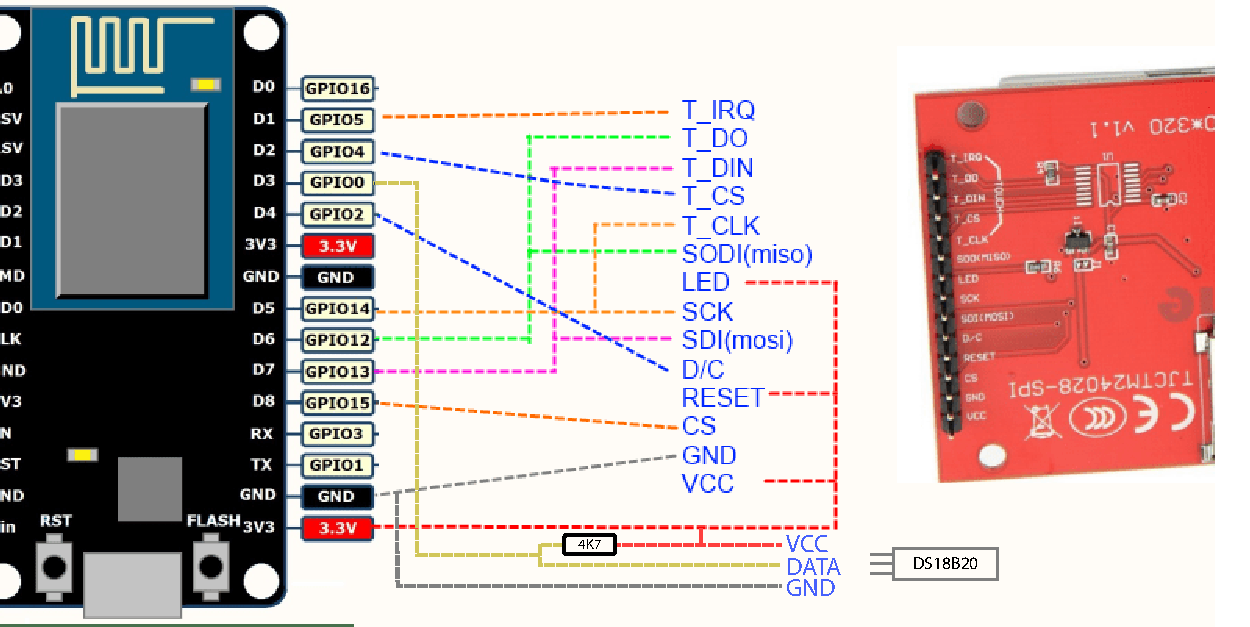
\includegraphics[width=0.7\textwidth]{img/wiring.pdf}
    \caption{\label{img-wiring}Zapojení řídící desky, displeje a senzoru teploty \cite{esp-wiring}}
\end{figure}

\subsection{Výroba} % fotky 
Jednotlivé součástky byly zapojeny dle diagramu na obrázku \ref{img-wiring}. Pro zařízení jsem navrhl krabičku na míru a následně ji vytiskl na 3D tiskárně. Výsledné zařízení je napájené pomocí micro usb, tedy stačí běžná nabíječka na telefon a teplotní senzor se připojuje pomocí konektoru kvůli jednodušší manipulaci. Dále bylo potřeba vytvořit program, který poběží na zařízení pro odesílání teploty do Platformy a bude zobrazovat informace (teplotu, čas) na displeji. Ukázka kódu \ref{code} obsahuje využití vytvořené knihovny v sekci \ref{library} pro napojení chytré udírny na Platformu. Výsledný program obsahuje tento kód obohacený o komunikaci s displejem a načtení času z internetu. Model krabičky a finální zdrojový kód naleznete na přiloženém médiu viz. příloha \ref{medium}.

\begin{figure}[htbp]
    \centering
    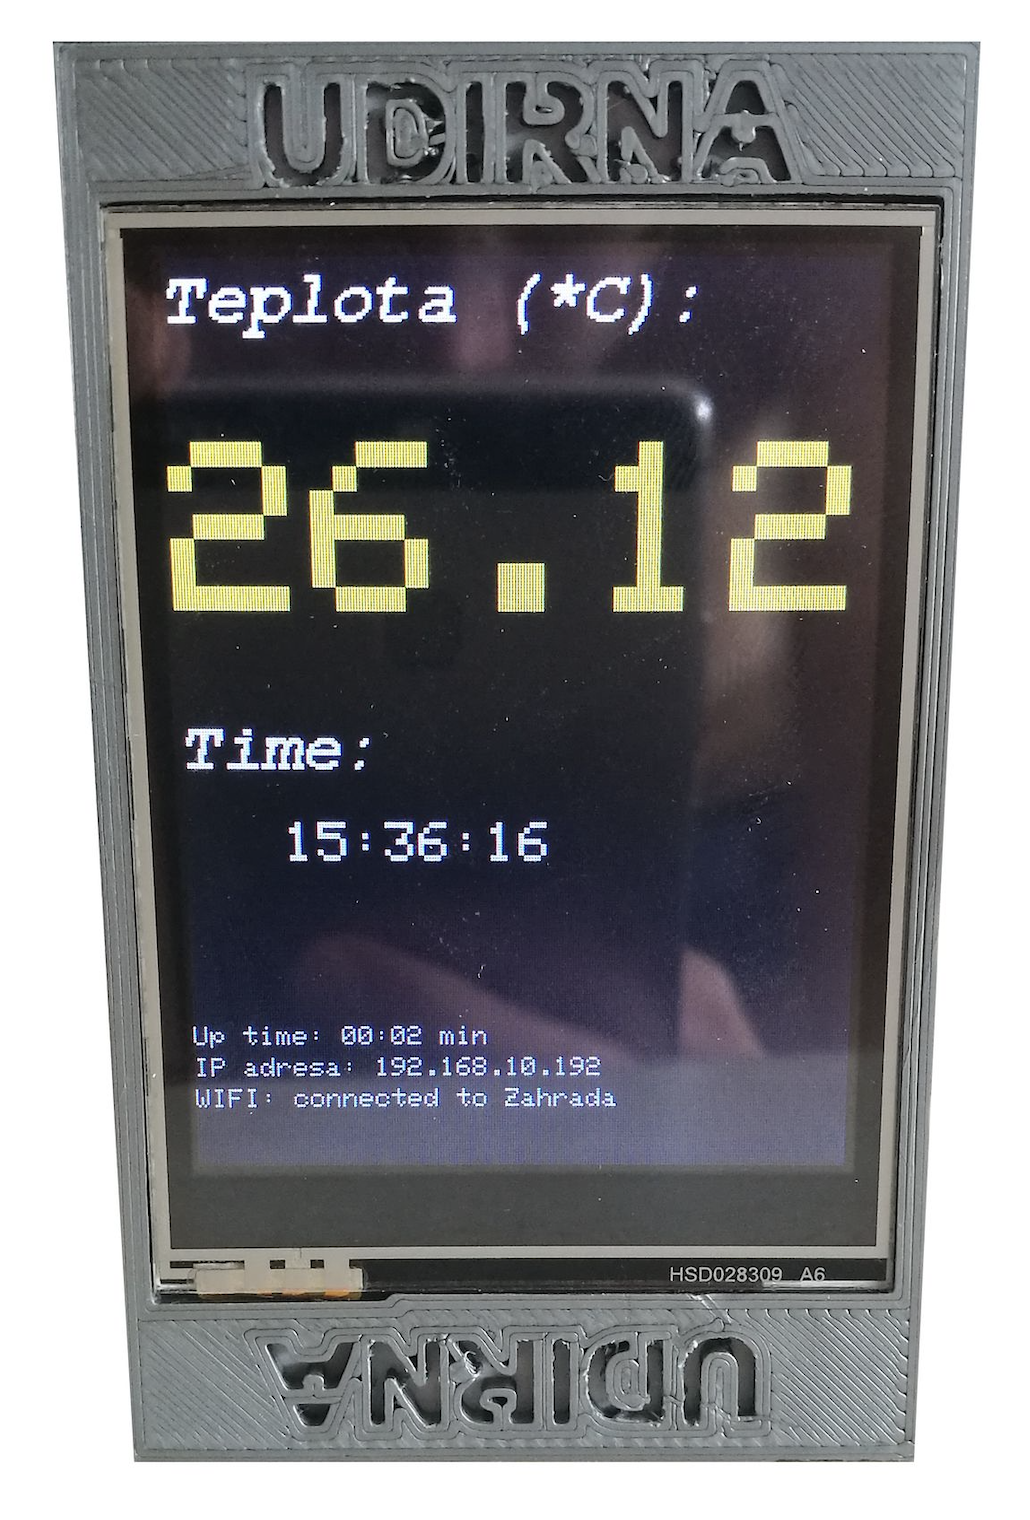
\includegraphics[width=0.5\textwidth]{img/smokehouse.png}
    \caption{\label{smokehouse}Finální verze výrobku}
\end{figure}

\begin{figure}[h!tb]
    \begin{minted}[linenos=true]{Arduino}
#include <IOTPlatforma.h>
#include <OneWire.h>
#include <DallasTemperature.h>

IOTPlatforma plat("Udírna");
OneWire oneWire(D3);
DallasTemperature sensors(&oneWire);
Property * propTemp;

void setup() {
    Node *node = plat.NewNode("sensor0", "Senzor", NodeType::SENSOR);
    propTemp = node->NewProperty("temperature", "Teplota", DataType::FLOAT);
    propTemp->setClass(PropertyClass::TEMPERATURE);
    propTemp->setUnit("°C");

    plat.start();
}

void loop() {
    plat.loop();

    sensors.requestTemperatures();
    float temp = sensors.getTempCByIndex(0);
    propTemp->setValue(String(temperature, 2).c_str());
    delay(1000);
}
\end{minted}
    \caption{\label{code}Kód pro odesílání teploty}
\end{figure}

\begin{figure}[htbp]
    \centering
    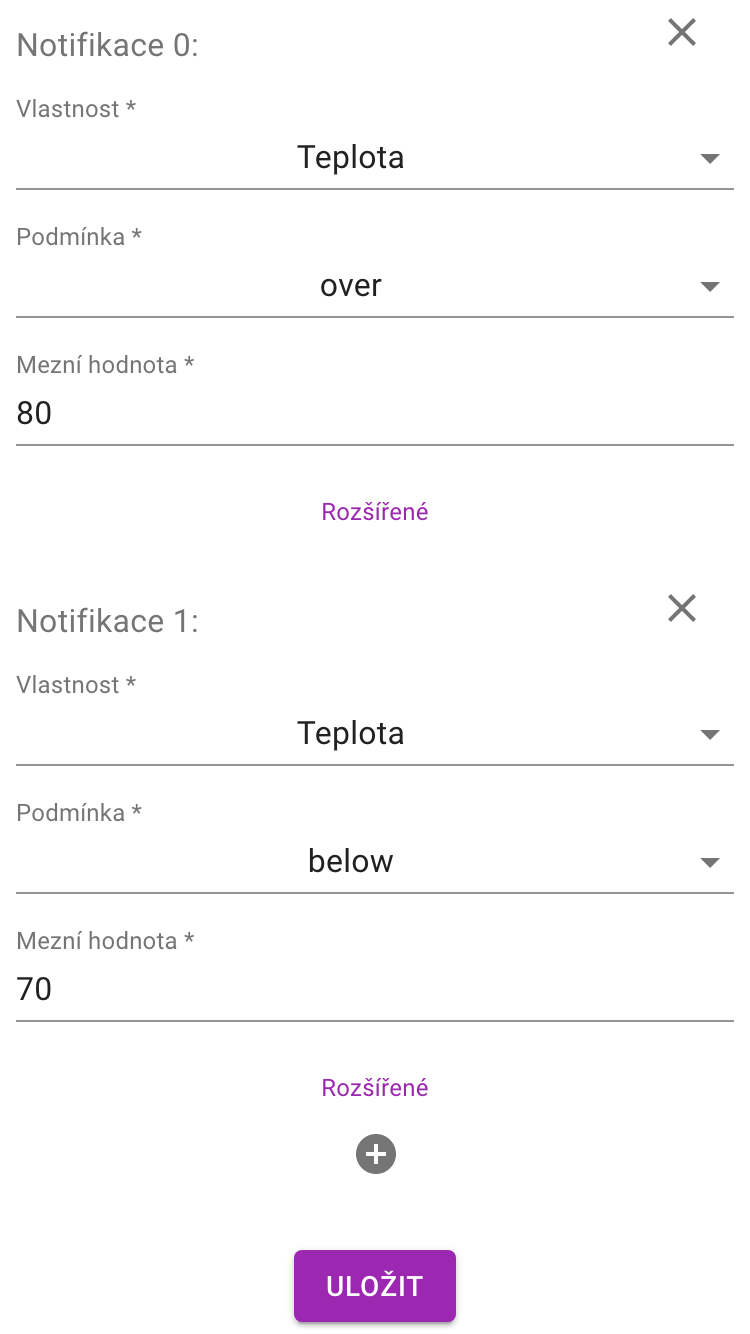
\includegraphics[width=0.5\textwidth]{img/notification_edit.png}
    \caption{Nastavení pravidel notifikací}
\end{figure}

\chapter{Testování}
Tato kapitola se zabývá testováním implemetovaného řešení nasazeného v produkčním prostředí. V první fázi je otestována stabilita řešení při velké zátěži a ve druhé intuitivnost uživatelského webového rozhraní. Produkční prostředí běží ve virtualizovaném serveru se systémem Debian (linux), přidělenými hardwarovými prostředky: CPU (5 vláken Ryzen 3600), 9~GB RAM, HDD (7200 otáček). Použitá verze NodeJS 12.22.1, MongoDB 4.2.13 a RabbitMQ 3.8.14.

\section{Zátěžové testování}
Obsloužit desítky připojených zařízení není s dnešním výkonným hardwarem žádný problém. Pro ověření chování řešení pod opravdu velkou zátěží - desítky paralelních požadavků a stovky připojených zařízení - jsem vytvořil automatizovaný test, kterému se definuje počet uživatelů a počet zařízení, které mezi uživatele má rozprostřít a o vše ostatní se test postará sám (pomocí HTTP požadavků stejně jako by uživatel interagoval přes webové rozhraní).

Prvně je vytvořen příslušný počet uživatelů a všechna virtuální zařízení (komunikující přes MQTT protokol stejně jako reálná). Všem uživatelům jsou načtena objevená zařízení, která jsou následně spárována a začínají odesílat data ze senzorů a jiných vlastností simulujících reálný provoz. Data se odesílají v náhodném rozmezí 50 - 60 vteřin, aby se provoz rozložil v čase. Test probíhal v následující konfiguraci:
\begin{itemize}
    \item počet uživatelů 25
    \item počet zařízení 250
    \item konfigurace zařízení - 2 senzory (teplota, vlhkost) a přepínač, data ze všech tří vlastností jsou odesílána paralelně
    \item počet paralelních API požadavků 10
\end{itemize}
Pro sledování zátěže databáze byl využit \uv{Free monitoring} \cite{free-monitoring}, který sleduje dobu provádění operací, jejich počet a vytížení disku. Pro sledování zátěže cpu jednotlivých procesů byl použit linuxový nástroj \textit{htop} a pro vykreslení grafu celkové zátěže cpu \textit{Kibana}. Protože se jedná o více jádrový stroj, tak vytížení cpu nemá maximum 100\,\%, ale pro každé jádro 100\,\%, tedy celkem 500\,\%. Test byl proveden celkově 3x pro ověření správnosti naměřených dat. Tabulka dat, ze kterých byl sestaven graf na obrázku \ref{cpu-usage} je umístěna na přiloženém médiu viz. příloha \ref{medium}.

\begin{figure}[htbp]
    \centering
    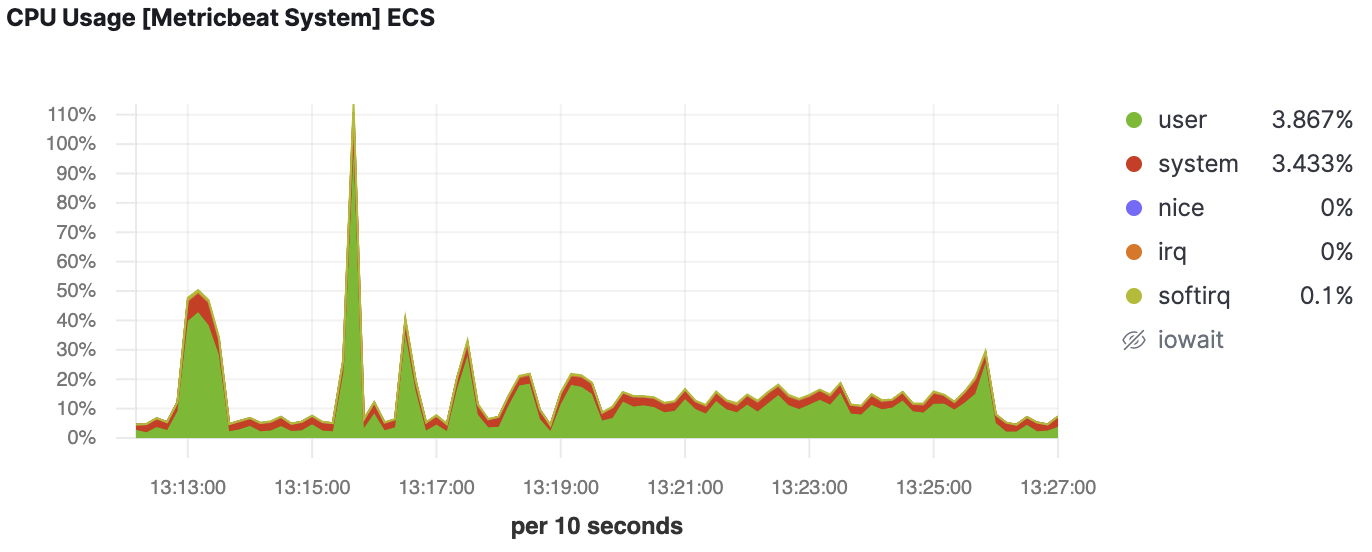
\includegraphics[width=\textwidth]{img/cpu_usage.png}
    \caption{\label{cpu-usage}Zátěž CPU během testu}
\end{figure}

První zvýšení trvající minutu je způsobeno zařízeními ohlašujícími svoje vlastnosti, což způsobilo velký počet zápisů do databáze. Druhé zvýšení ve 13:15:40 trvající 20 vteřin způsobilo přidání jednotlivých zařízení uživatelům (a jejich spárování). Následujících 10\,min trvající zatížení bylo způsobeno tím, že zařízení odesílají data ze svých vlastností. Závěrečná několika vteřinová zvýšená zátěž ve 13:25:50 je dána odesláním informace o odpojení ze všech zařízení. V průběhu testu byla průměrná doba vyřízení databázové operace 0,24 ms, zátěž cpu databází 8 \%, procesem platformy 6 \% a zátěž disku přibližně 2 \%. V průběhu celého testu byla platforma aktivně využívána uživatelem přes webové rozhraní k ovládání fyzických zařízení a po celou dobu vše reagovalo ihned bez jakéhokoliv zpoždění, ani průměrná doba zpracování RESTful požadavku nebyla významně ovlivněna. Z výsledku testu tedy vyplývá, že platforma zvládne bez jakýchkoliv problémů obsloužit stovky zařízení bez negativního dopadu na výkon.


% popsat které části jsou náročné na DB maybe? Kolik DB query bylo během testu, čím jsem monitoroval prostředky, query max time, cpu usage

% protože se jedná o více jádrový stroj, tak % vytížení nemají max 100% ale 500%, protože 5 jader
% začátek - velký nápor trvající 1min, cpu až 100%, IOWait 80%, disk up to 60%
% průběh posílání dat - cpu - mongo 6%, node 6%
%                       - disk 1,5%
% za celou dobu doba provedení operace DB avg 0.12 ms, maximum 180 doc updated za sec, 
% v průběhu jsem používal platformu a ovládal fyzická zařízení, která reagovala ihned a doba provedení api requestů byla stejná jako bez zatížení
% provedeny byly 3 testy s rozmezím 1 hodina, aby se minimalizoval případný dopad cachen na výkon

% z testy je vidět největší zátěž první minutu, kdy zařízení paralelně ohlašují svoje vlastnosti, následná dlouhodobá zátěž je způsobena neustálým odesíláním naměřených dat ze všech zařízení.

% \section{Zotavení po nenadálé události}

\section{Uživatelské testování}
Za pomoci uživatelského testování byla ověřena intuitivnost uživatelského prostředí. Cílem bylo zjistit, zda uživatelé zvládnou vykonat základní úkony bez pomoci a zjistit jejich náročnost.

Každý uživatel dostal uživatelskou příručku (příloha \ref{user-guide}), přístup k již naprogramovanému zařízení, které ovládalo led světla a měřilo teplotu, a nakonec seznam úkonů, které mají vykonat a zpětně je ohodnotit na stupnici od jedné do pěti (pět je nejhorší). První tester byl muž, věk 49, se zájmem o techniku. Druhý byl také muž, věk 30, s ekonomickým vzděláním.


\begin{figure}
    \centering
    % \begin{adjustbox}{angle=-90}
    % \begin{center} % pro addony přidat poznámku 324 obsahuje 2585 věcí
    \begin{tabular}{ | l | c | c | }
        \hline
        Úkon                           & Uživatel 1 & Uživatel 2 \\
        \hline
        Připojte nové zařízení         & 4          & 3          \\
        \hline
        Zapněte led světla             & 1          & 1          \\
        \hline
        Podívejte se na průběh teplotu & 2          & 2          \\
        \hline
        Změňte umístění zařízení       & 1          & 1          \\
        \hline
        Zařízení odstraňte             & 1          & 1          \\
        \hline
    \end{tabular}
    \caption{Hodnocení jednotlivých testerů}
\end{figure}

V průběhu testování se ukázal jako nejvíce problematický první krok, ve kterém uživatel zadává v kaptivním portále údaje k připojení na domácí Wifi a své uživatelské jméno k platformě. Zařízení občas ohlásilo chybu připojení k Wifi i při správně zadaných údajích. Ostatní části testu již probíhaly bez jakéhokoliv problému. Dle závěrečného hodnocení se rozhraní ukázalo jako uživatelsky velmi přívětivé a zařízení po úspěšném připojení k Wifi pracovalo již naprosto spolehlivě. Po ukončení testu byly uživatelé v nezávazném rozhovoru dotázáni na možná vylepšení. Z rozhovoru vyplynulo doporučení do budoucna k vytvoření interaktivního průvodce, který by při první návštěvě vysvětlil pokročilejší funkce.

Po bližším zkoumání problematického připojení byl zjišten problém s knihovnou \textit{WifiManager}, která má na starosti vytvoření kaptivního portálu a následné připojení na Wifi. Aktuální verze této knihovny prochází rapidním vývojem s nedostatečnou dokumentací aktuálních funkcí. Nepodařilo se identifikovat, zda je problém se špatným využitím této knihovny či v implementaci knihovny samotné. Pro nalezení řešení bude kontaktován autor knihovny a v případě neúspěchu je možnost využití jiné knihovny implementující podobnou funkcionalitu např. \textit{IotWebConf}.

\begin{conclusion}
    Cílem této práce bylo navrhnout a implementovat vlastní IoT Platformu. Byla provedena rešerže a porovnání čtyř Platforem: Bynk, ThingSpeak, Home Assistant a OpenHab. Pro návrh vlastního řešení byla vytvořena koncepce, kterou měla být otevřená více uživatelská Platforma pro připojení různorodých zařízení vyrobených kutily a technickými entuziasty. Základním pilířem celého řešení mělo být vytvoření schématu, dle kterého každé zařízení popíše své schopnosti a uživateli se následně zobrazní příslušné rozhraní vygenerované ná základě jeho dovedností. Každý uživatel měl mít k dispozici vlastní sféru v rámci, které jeho zařízení komunikují.

    Všech definovaných cílů bylo dosaženo. Bylo vytvořené schéma na protokolu MQTT, které umožňuje zařízením přesně popsat své dovednosti, na jejichž základě je vykresleno uživatelské rozhraní. Jsou podporovány různé kombinace vlasnosti od úzce specifických prvků jako přepínač až po obecné odeslání textu. Bylo vytvořeno intuitivní webové rozhraní, které umožňuje interakci se zařízeními, vizualizaci některých dat a nastavení push notifikací. Byla vytvořena knihovna pro koncová zařízení, umožňující snadné napojení na Platformu a vzniklo zařízení, na kterém bylo demonstrováno její použití. Řešení bylo nasazeno a podrobeno zátěžovému a uživatelskému testování, ve kterém se prokázala schopnost obsloužit stovky zařízení a intuitivnost celého rozhraní.

    Celé řešení bude zveřejněno a uvolněno pod licencí GPLv3 na stránce XXX.
\end{conclusion}

\bibliographystyle{csn690}
\bibliography{mybibliographyfile}

\appendix

\chapter{Seznam použitých zkratek}
% \printglossaries
\begin{description}
    \item[ACL]
    \item[DIY]
    \item[SPA]
    \item[RESTful]
\end{description}

\chapter{Obrázky}
\begin{figure}[htbp]
    \centering
    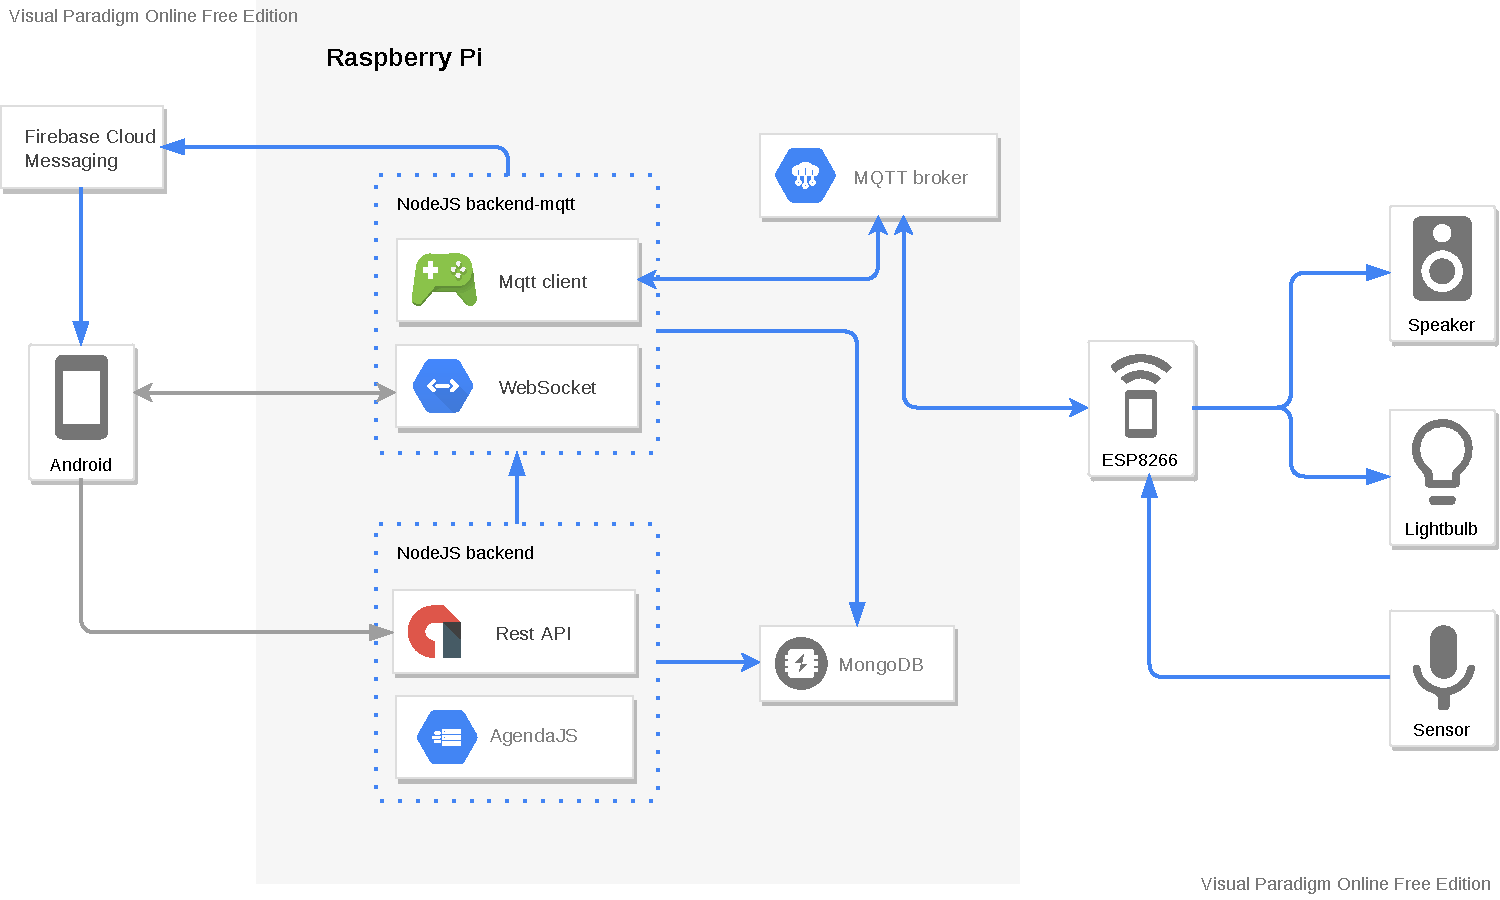
\includegraphics[width=\textwidth]{img/architecture.pdf}
    \caption{Náhled fyzické architektury}
\end{figure}

\begin{figure}[htbp]
    \centering
    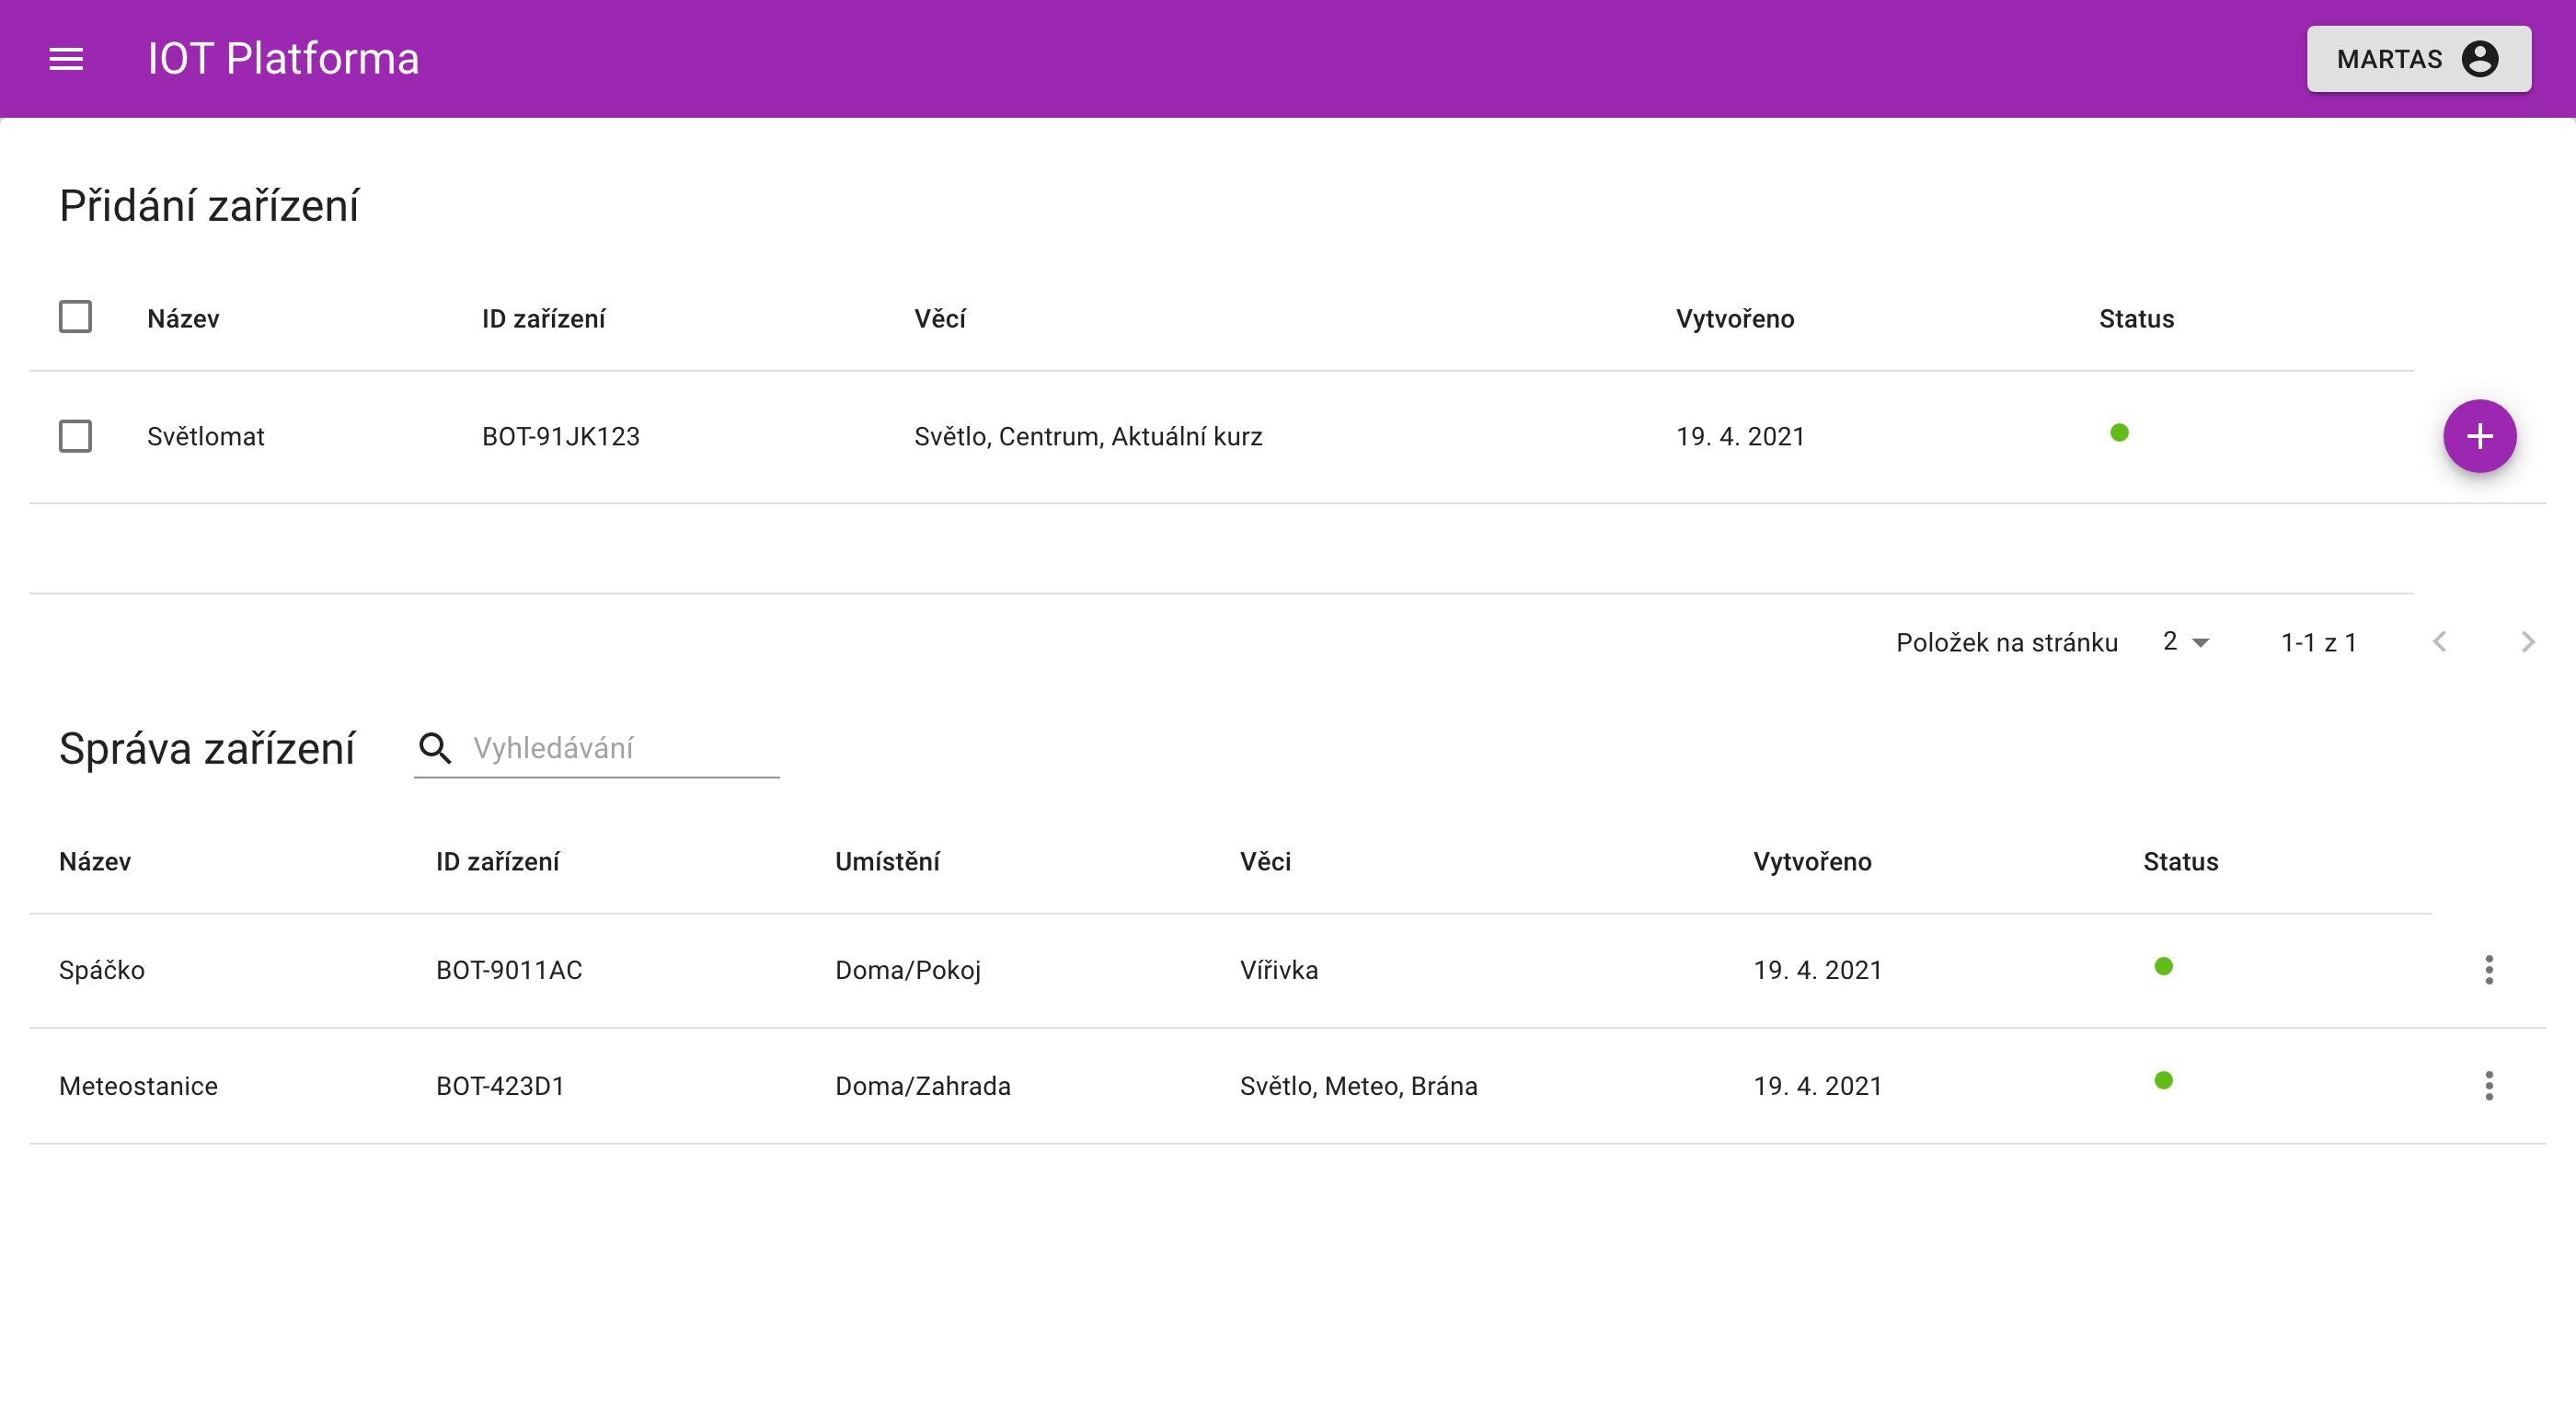
\includegraphics[width=\textwidth]{img/screens/deviceManagement2.png}
    \caption{Ukázka rozhraní - správa zařízení}
\end{figure}

\begin{figure}
    \centering
    \begin{subfigure}{.5\textwidth}
        \centering
        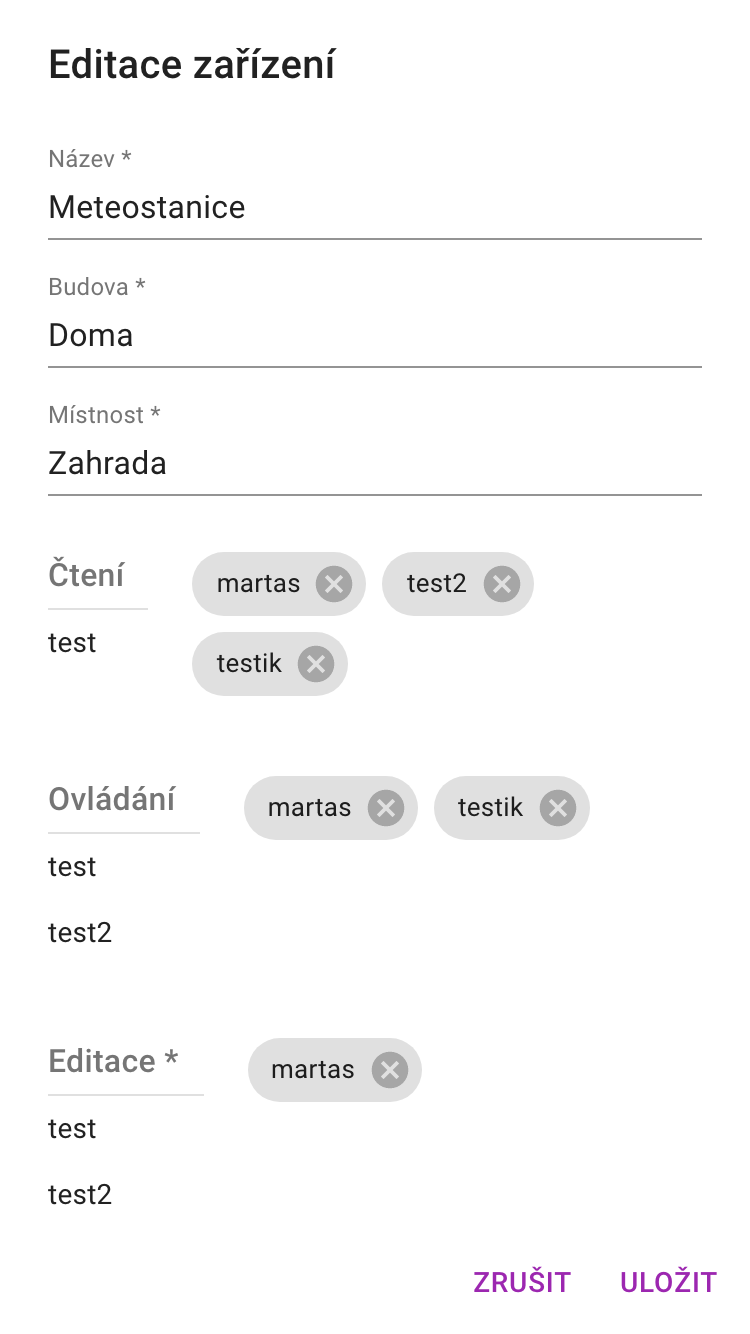
\includegraphics[width=.7\linewidth]{img/screens/editDevice.png}
        \caption{Zobrazení místností}
    \end{subfigure}%
    \begin{subfigure}{.5\textwidth}
        \centering
        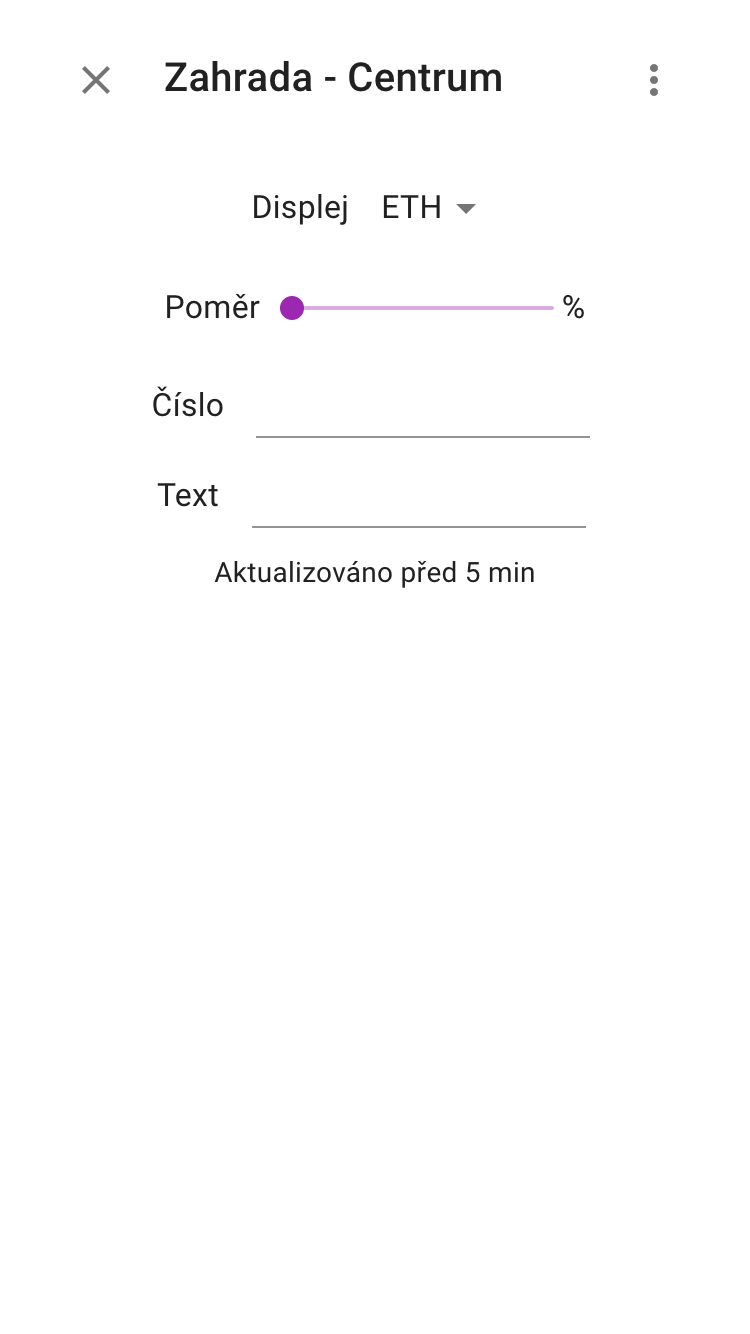
\includegraphics[width=.7\linewidth]{img/screens/generic.png}
        \caption{Zobrazení místnosti}
    \end{subfigure}
    \caption{Ukázka rozhraní}
\end{figure}



\begin{figure}[htbp]
    \centering
    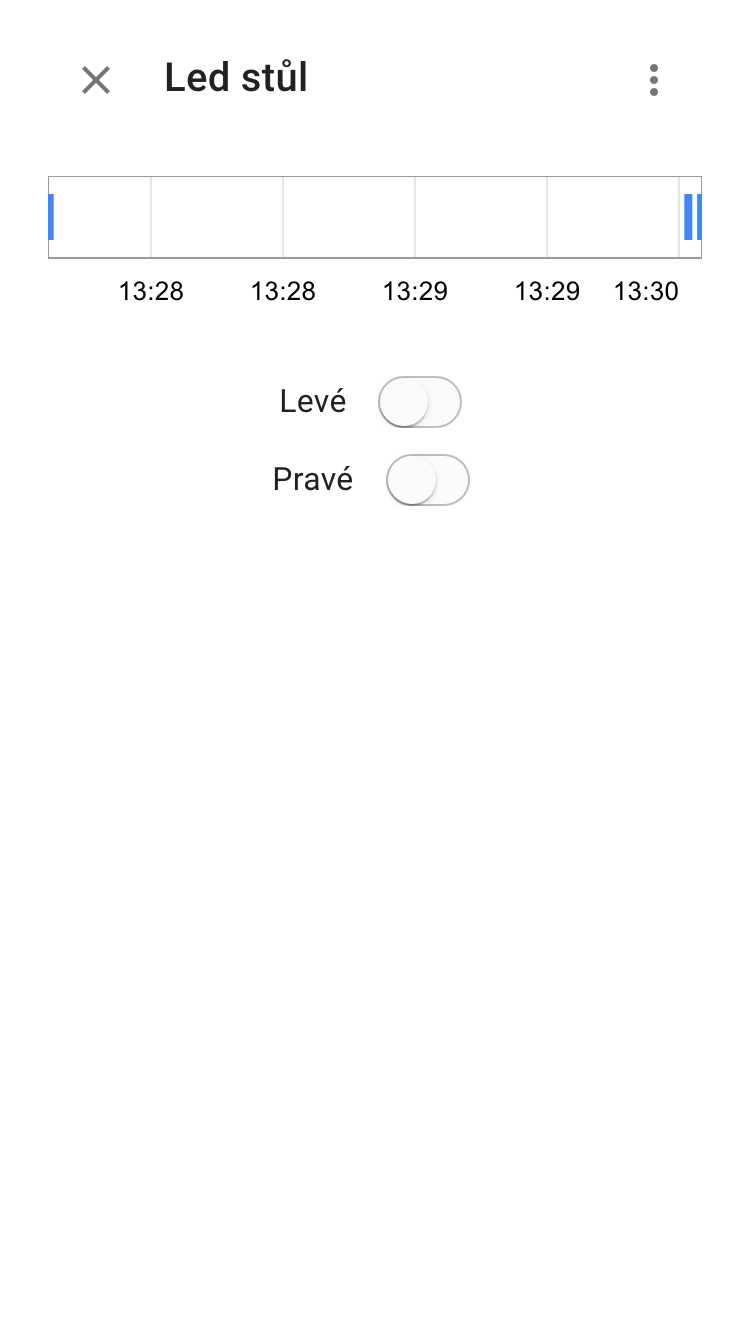
\includegraphics[width=0.5\textwidth]{img/screens/led.png}
    \caption{Ukázka rozhraní - věc typu switch}
\end{figure}

\chapter{Uživatelská příručka}\label{user-guide}
\begin{enumerate}
    \item Zařízení zapněte.
    \item Přihlaste se, případně zaregistrujte k Platformě na stránce \\
          \href{https://dev.iotplatforma.cloud}{https://dev.iotplatforma.cloud}.
    \item Připojte svůj telefon/notebook k wifi s názvem ,,Nastav mě”.
    \item Budete upozorněni na nutnost přihlášení k síti, otevřete tuto možnost a zobrazí se Vám webová stránka. Klikněte na ,,Configure wifi”, kde budete vyzváni k zadání údajů pro připojení k Vaší domácí Wifi. Dále zadejte Vaše uživatelské jméno, které používáte pro přihlášení k Platformě a klikněte na tlačítko ,,Save”. Zařízení se nyní restartuje a připojí k wifi.
    \item Pokud v předchozím bodu byly zadány nesprávné údaje, tak se znovu vytvoří wifi ,,Nastav mě”, v tom případě opakujte postup od bodu 3.
    \item zařízení. Na začátku se objeví sekce “Přidat zařízení”, kde budete mít nové zařízení a to si přidejte pomocí tlačítka plus. Budete vyzváni k zadání umístění zařízení.
    \item Nyní na stránce Zařízení již můžete zařízení sledovat a ovládat.66
\end{enumerate}
% % % % % % % % % % % % % % % % % % % % % % % % % % % % 
% % Tuto kapitolu z výsledné práce ODSTRAŇTE.
% % % % % % % % % % % % % % % % % % % % % % % % % % % % 
% 
% \chapter{Návod k~použití této šablony}
% 
% Tento dokument slouží jako základ pro napsání závěrečné práce na Fakultě informačních technologií ČVUT v~Praze.
% 
% \section{Výběr základu}
% 
% Vyberte si šablonu podle druhu práce (bakalářská, diplomová), jazyka (čeština, angličtina) a kódování (ASCII, \mbox{UTF-8}, \mbox{ISO-8859-2} neboli latin2 a nebo \mbox{Windows-1250}). 
% 
% V~české variantě naleznete šablony v~souborech pojmenovaných ve formátu práce\_kódování.tex. Typ může být:
% \begin{description}
% 	\item[BP] bakalářská práce,
% 	\item[DP] diplomová (magisterská) práce.
% \end{description}
% Kódování, ve kterém chcete psát, může být:
% \begin{description}
% 	\item[UTF-8] kódování Unicode,
% 	\item[ISO-8859-2] latin2,
% 	\item[Windows-1250] znaková sada 1250 Windows.
% \end{description}
% V~případě nejistoty ohledně kódování doporučujeme následující postup:
% \begin{enumerate}
% 	\item Otevřete šablony pro kódování UTF-8 v~editoru prostého textu, který chcete pro psaní práce použít -- pokud můžete texty s~diakritikou normálně přečíst, použijte tuto šablonu.
% 	\item V~opačném případě postupujte dále podle toho, jaký operační systém používáte:
% 	\begin{itemize}
% 		\item v~případě Windows použijte šablonu pro kódování \mbox{Windows-1250},
% 		\item jinak zkuste použít šablonu pro kódování \mbox{ISO-8859-2}.
% 	\end{itemize}
% \end{enumerate}
% 
% 
% V~anglické variantě jsou šablony pojmenované podle typu práce, možnosti jsou:
% \begin{description}
% 	\item[bachelors] bakalářská práce,
% 	\item[masters] diplomová (magisterská) práce.
% \end{description}
% 
% \section{Použití šablony}
% 
% Šablona je určena pro zpracování systémem \LaTeXe{}. Text je možné psát v~textovém editoru jako prostý text, lze však také využít specializovaný editor pro \LaTeX{}, např. Kile.
% 
% Pro získání tisknutelného výstupu z~takto vytvořeného souboru použijte příkaz \verb|pdflatex|, kterému předáte cestu k~souboru jako parametr. Vhodný editor pro \LaTeX{} toto udělá za Vás. \verb|pdfcslatex| ani \verb|cslatex| \emph{nebudou} s~těmito šablonami fungovat.
% 
% Více informací o~použití systému \LaTeX{} najdete např. v~\cite{wikilatex}.
% 
% \subsection{Typografie}
% 
% Při psaní dodržujte typografické konvence zvoleného jazyka. České \uv{uvozovky} zapisujte použitím příkazu \verb|\uv|, kterému v~parametru předáte text, jenž má být v~uvozovkách. Anglické otevírací uvozovky se v~\LaTeX{}u zadávají jako dva zpětné apostrofy, uzavírací uvozovky jako dva apostrofy. Často chybně uváděný symbol "{} (palce) nemá s~uvozovkami nic společného.
% 
% Dále je třeba zabránit zalomení řádky mezi některými slovy, v~češtině např. za jednopísmennými předložkami a spojkami (vyjma \uv{a}). To docílíte vložením pružné nezalomitelné mezery -- znakem \texttt{\textasciitilde}. V~tomto případě to není třeba dělat ručně, lze použít program \verb|vlna|.
% 
% Více o~typografii viz \cite{kobltypo}.
% 
% \subsection{Obrázky}
% 
% Pro umožnění vkládání obrázků je vhodné použít balíček \verb|graphicx|, samotné vložení se provede příkazem \verb|\includegraphics|. Takto je možné vkládat obrázky ve formátu PDF, PNG a JPEG jestliže používáte pdf\LaTeX{} nebo ve formátu EPS jestliže používáte \LaTeX{}. Doporučujeme preferovat vektorové obrázky před rastrovými (vyjma fotografií).
% 
% \subsubsection{Získání vhodného formátu}
% 
% Pro získání vektorových formátů PDF nebo EPS z~jiných lze použít některý z~vektorových grafických editorů. Pro převod rastrového obrázku na vektorový lze použít rasterizaci, kterou mnohé editory zvládají (např. Inkscape). Pro konverze lze použít též nástroje pro dávkové zpracování běžně dodávané s~\LaTeX{}em, např. \verb|epstopdf|.
% 
% \subsubsection{Plovoucí prostředí}
% 
% Příkazem \verb|\includegraphics| lze obrázky vkládat přímo, doporučujeme však použít plovoucí prostředí, konkrétně \verb|figure|. Například obrázek \ref{fig:float} byl vložen tímto způsobem. Vůbec přitom nevadí, když je obrázek umístěn jinde, než bylo původně zamýšleno -- je tomu tak hlavně kvůli dodržení typografických konvencí. Namísto vynucování konkrétní pozice obrázku doporučujeme používat odkazování z~textu (dvojice příkazů \verb|\label| a \verb|\ref|).
% 
% \begin{figure}\centering
% 	
\includegraphics[width=0.5\textwidth, angle=30]{cvut-logo-bw}
% 	\caption[Příklad obrázku]{Ukázkový obrázek v~plovoucím prostředí}\label{fig:float}
% \end{figure}
% 
% \subsubsection{Verze obrázků}
% 
% % Gnuplot BW i barevně
% Může se hodit mít více verzí stejného obrázku, např. pro barevný či černobílý tisk a nebo pro prezentaci. S~pomocí některých nástrojů na generování grafiky je to snadné.
% 
% Máte-li například graf vytvořený v programu Gnuplot, můžete jeho černobílou variantu (viz obr. \ref{fig:gnuplot-bw}) vytvořit parametrem \verb|monochrome dashed| příkazu \verb|set term|. Barevnou variantu (viz obr. \ref{fig:gnuplot-col}) vhodnou na prezentace lze vytvořit parametrem \verb|colour solid|.
% 
% \begin{figure}\centering
% 	\includegraphics{gnuplot-bw}
% 	\caption{Černobílá varianta obrázku generovaného programem Gnuplot}\label{fig:gnuplot-bw}
% \end{figure}
% 
% \begin{figure}\centering
% 	\includegraphics{gnuplot-col}
% 	\caption{Barevná varianta obrázku generovaného programem Gnuplot}\label{fig:gnuplot-col}
% \end{figure}
% 
% 
% \subsection{Tabulky}
% 
% Tabulky lze zadávat různě, např. v~prostředí \verb|tabular|, avšak pro jejich vkládání platí to samé, co pro obrázky -- použijte plovoucí prostředí, v~tomto případě \verb|table|. Například tabulka \ref{tab:matematika} byla vložena tímto způsobem.
% 
% \begin{table}\centering
% 	\caption[Příklad tabulky]{Zadávání matematiky}\label{tab:matematika}
% 	\begin{tabular}{|l|l|c|c|}\hline
% 		Typ		& Prostředí		& \LaTeX{}ovská zkratka	& \TeX{}ovská zkratka	\tabularnewline \hline \hline
% 		Text		& \verb|math|		& \verb|\(...\)|	& \verb|$...$|		\tabularnewline \hline
% 		Displayed	& \verb|displaymath|	& \verb|\[...\]|	& \verb|$$...$$|	\tabularnewline \hline
% 	\end{tabular}
% \end{table}
% 
% % % % % % % % % % % % % % % % % % % % % % % % % % % % 

\chapter{Obsah přiloženého CD}
\label{medium}
\begin{figure}
    \dirtree{%
        .1 readme.md\DTcomment{stručný popis obsahu CD}.
        .1 smokehouse\DTcomment{adresář se spustitelnou formou implementace}.
        .2 library.
        .3 IOT\_platforma\_v3\DTcomment{implementovaná knihovna}.
        .2 models\DTcomment{stl modely pro 3D tisk}.
        .2 src.
        .3 main.cpp\DTcomment{zdrojový kód pro chytrou udírnu}.
        .1 platforma\DTcomment{implementovaná platforma}.
        .2 packages\DTcomment{zdrojové kódy implementace}.
        .2 readme.md\DTcomment{instalační příručka}.
        .1 thesis\DTcomment{zdrojová forma práce ve formátu \LaTeX{}}.
        .1 thesis.pdf\DTcomment{text práce ve formátu PDF}.
    }
\end{figure}

\end{document}
